\documentclass[a4paper]{article}
\usepackage{fullpage}
\usepackage{enumerate}
\usepackage[T1,T2A]{fontenc}
\usepackage[utf8]{inputenc}
\usepackage[bulgarian]{babel}
\usepackage{soul}
\usepackage{graphicx}
\usepackage{usecases}

%\renewcommand{\thesection}{\Roman{section}} 
%\renewcommand{\thesubsection}{\thesection.\Roman{subsection}}

\begin{document}

%\title{\sc{Информационна система на агенция за недвижими имоти}\\Обобщен доклад.}
\title{Информационна система на агенция за недвижими имоти\\Обобщен доклад}
\author{Екип $\pi \approx 3.1$}

\maketitle

\begin{center}

\begin{tabular}{r|l}
%\hline
71469	& Георги Димов \\ %\hline
71473	& Цветан Цветанов \\ %\hline
71488	& Антон Дудов \\ %\hline
71490	& Венцислав Конов \\ %\hline
71492	& Александър Танков \\ %\hline
71508	& Красимир Тренчев \\ %\hline
71512	& Александър Велин \\ %\hline
71524	& Анджелика Туджарска \\ %\hline
71529	& Александър Бранев \\ %\hline
855240	& Мартин Стоев \\ %\hline
\end{tabular}

\end{center}

\clearpage

\tableofcontents

\clearpage

\begin{table}[h]
\centering
\label{my-label}
\begin{tabular}{|p{1.7cm}|p{1cm}|p{11cm}|p{1.6cm}|}
\hline
Дата       & Част & Промяна                                                                                             & От        \\ \hline
\hline
2016-05-14 & I    & Променен модел на дейностите на Брокер                                                              					& В. Конов  \\ \hline
2016-05-14 & I    & Променен модел на дейностите на Регистриран потребител                                              					& А. Бранев \\ \hline
2016-05-14 & I    & Добавени описания на дейностите и отговорностите към модела на 
дейностите на Регистриран потребител 
					& А. Бранев \\ \hline
2016-05-14 & I    & Премахнати референции към конкретни интерфейсни елементи                                            					& М. Стоев  \\ \hline
2016-05-14 & I    & Променено описание на чат системата                                                                 					& В. Конов  \\ \hline
2016-05-26 & II	  & Променен шаблон за потребителските случаи																& А. Велин	\\ \hline
2016-05-27 & II	  & Променен модел на потребителските случаи																& А. Велин	\\ \hline
2016-05-27 & II	  & Променено описание на категоризацията на потребителските случаи											& А. Велин	\\ \hline
2016-05-27 & II	  & Отразени коментарите в пълното описание на потребителските случаи
					& А. Велин	\\ \hline
2016-06-04 & II	  & Нанесени липсващите стойности в таблицата с разпределението на времето
					& А. Велин	\\ \hline
\end{tabular}
\caption{Списък на промените в документа}
\end{table}

\clearpage

\part{Приложение на принципите за контекстуално проектиране} \label{cd}
\setcounter{section}{0}
\setcounter{table}{0}

\section{Обща представа за системата} %FIXME ?
        
Трябва да се проектира информационна система за стартираща агенция за недвижими имоти, която до момента не е използвала никакви системи и няма съществуващи към момента бизнес процеси. Описаната тук система е според изискванията на собственика на агенцията.

Целта на информационната система е да осигури уеб интерфейс, чрез който брокерите могат да управляват своите обяви за недвижими имоти, а клиентите на агенцията (наематели и купувачи) да имат гъвкав и удобен интерфейс за търсене на обяви за имоти по различни критерии, както и да инициират комуникация с брокера. Връзката между собствениците на имоти и брокерите ще се осъществява извън рамките на системата.

Всички счетоводни и финансови процеси в агенцията не са предмет на информационната система.

\section{Интервюта}
В рамките на проведените интервюта бе събрана информация от следните потребители:

\begin{center}
\begin{tabular}{|l|l|}
\hline
Борислав Арнаудов & Собственик на стартираща агенция за недвижими имоти \\
\hline
\end{tabular}
\end{center}

На първото интервю (проведено на 2016-03-18 от 16:00 до 17:30 в зала 01 на ФМИ) присъстваха от страна на клиента:
\begin{itemize}
\item Борислав Арнаудов
\end{itemize}
и от страна на студентите:
\begin{itemize}
\item Георги Димов
\item Цветан Цветанов
\item Антон Дудов
\item Венцислав Конов
\item Александър Танков
\item Красимир Тренчев
\item Александър Велин
\item Анджелика Туджарска
\item Александър Бранев
\item Мартин Стоев
\end{itemize}

На второто интервю (2016-04-01 от 09:00 до 10:30 в САП България) присъстваха от страна на клиента:
\begin{itemize}
\item Борислав Арнаудов
\end{itemize}
и от страна на студентите:
\begin{itemize}
\item Георги Димов
\item Цветан Цветанов
\item Венцислав Конов
\item Александър Танков
\item Красимир Тренчев
\item Александър Велин
\item Анджелика Туджарска
\item Александър Бранев
\end{itemize}

По време на интервютата бяха изяснени изискванията към системата.

\subsection{Функционалност на системата}

\subsubsection{Достъп и акаунти}
% Достъп и акаунти

Системата трябва да поддържа както анонимен (публичен) достъп, така и достъп на потребители, които имат създаден акаунт в системата. Всеки акаунт има следните данни:
	\begin{itemize}
	\item username (задължителен);
	\item парола (задължителен);
	\item email (задължителен);
	\item име (задължителен);
	\item телефон;
	\item снимка.
	\end{itemize}

Брокерските профили имат натрупан до момента рейтинг на брокера.
				
Автентифицирането на потребители да се извършва от допълнителна система, свързана с основната. Данните за потребителите да се пазят на различен от основния сървър. Паролите да бъдат криптирани чрез използване на ``сол'' и силен хеширащ алгоритъм. 

\subsubsection{Роли}
% Роли
Системата трябва да поддържа следните роли:
	\begin{itemize}
	\item {нерегистриран потребител - има права да:
		\begin{itemize}
		\item търси и разглежда обяви в сайта;
		\item споделя обяви в социалните мрежи;
		\item си регистрира акаунт, с потвърждение по email, за да се гарантира вярност на вписания адрес;
		\item използва контакт формата за изпращане на съобщение към брокерите;
		\item използва чат системата, като не му се запазва log на разговора.
		\end{itemize}
	}
	\item {регистриран потребител - има права да:
		\begin{itemize}
		\item прави всички неща, които може нерегистриран потребител, освен регистрация на акаунт;
		\item използва чат системата, като се запазва log на разговора;
		\item ``запазва'' обяви, които е харесал в профила си;
		\item променя личните си данни;
		\item поиска ресет на паролата си (през email);
		\item подаде заявка, че иска да стане брокер.
		\end{itemize}
	}
	\item {брокер - има права да:
		\begin{itemize}
		\item прави всички неща, които може регистриран потребител;
		\item създава обяви за имоти;
		\item редактира и премахва своите обяви за имоти;
		\item променя състоянието на своите обяви (активни, неактивни, създадени);
		\item променя статуса на своя обява (нормална, VIP);
		\item комуникира през чат системата с други потребители, ако те са инициирали комуникацията;
		\item получава съобщения през контакт формата към дадена обява;
		\item вижда точният адрес на имота в обявите (както собствени, така и на други брокери);
		\item вижда контактната информация за собствениците на имотите в  обявите (както собствени, така и на други брокери);
		\item има право да вижда данни на даден потребител (username, email, име, телефон, снимка).
		\end{itemize}
	}
	\item {администратор (вграден в системата сервизен акаунт, единствен):
		\begin{itemize}
		\item прави всички неща, които може регистриран потребител;
		\item има право да вижда списък на потребителите в системата;
		\item има право да разглежда личните данни на потребителите (username, email, име, телефон, снимка);
		\item няма право да променя личните данни на потребителите (username, парола, email, име, телефон, снимка);
		\item има право да одобрява заявки на регистрирани потребители за промяна на статуса им към ``брокер'';
		\item има право да премахва статуса ``брокер'' от акаунти, след като е асоциирал обявите му с други брокери;
		\item има право да премахва акаунти от системата, без сервизните такива (администратор, одитор);
		\item няма право да редактира съдържанието на обява;
		\item има право да премахва обяви;
		\item има право да променя статуса на обява (нормална, VIP);
		\item има право да променя състоянието на обява (активна, неактивна) (при премахване или промяна на статуса/състоянието на обява се нотифицира брокера - собственик на обявата);
		\item има право да променя боркера-собственик на обява;
		\item получава копие от съобщенията, изпратени през контакт формата;
		\item препраща получено съобщене (от контакт форма) към брокер.
		\end{itemize}
	}
	\item одитор (вграден в системата сервизен акаунт, единствен) -- има права само да чете одит лога.
	\end{itemize}

\subsubsection{Обяви}

Обявите се създават, редактират и премахват от брокер. Администраторът има право да редактира и премахва обявите на всички брокери.	Обявите могат да бъдат активни или неактивни, като обикновенните потребители (нерегистрирани и регистрирани) виждат само активните обяви, докато неактивните обяви са видими само за брокерите и администратора.
Обявите могат да бъдат нормални или VIP. Този статус може да се променя само ръчно от брокерите и администратора.
Обявите съдържат следните данни:
	\begin{itemize}
	\item идентификатор на брокер;
	\item натрупан до момента рейтинг на обявата;
	\item активна/неактивна обява; 
	\item нормална/VIP обява;
	\item {характеристики на имота:
		\begin{itemize}
		\item местоположение - град, квартал, улица и номер, номер на блок;
		\item детайлно местоположение - град, квартал, улица и номер, номер на блок, вход, етаж, апартамент;
		\item площ в квадратни метри;
		\item тип на цената (месечен наем/цена за закупуване), валута (BGN, USD, EUR), цена;
		\item тип на имота - апартамент, къща, гараж, парцел;
		\item {специфични характеристики според типа:
			\begin{itemize}
			\item апартамент -- тип (едностаен, двустаен, тристаен, многостаен, мезонет, студио), етаж, изложение, година и тип на строителството, прилежащи имоти (мазета, гаражи) и общи части, обзавеждане, интернет, ТЕЦ, СОТ, телефон, ток, вода;
			\item къща -- застроена и дворна площ, брой етажи, прилежащи имоти (мазета, гаражи),	обзавеждане, интернет, ТЕЦ, СОТ, телефон, ток, вода;
			\item гараж -- ток, вода;
			\item парцел -- тип (в регулация, земеделска земя), ток, вода.
			\end{itemize}
		}
		\end{itemize}
	}
	\item текстово поле -- свободно описание на обявата, до 5 KB. Полето трябва да позволява въвеждането на символи за нов ред;
	\item снимки и скици -- binary формат, до 20 броя общо, всяка с размер до 1 MB, минимум една снимка и една скица; 
	\item географски данни, описващи точната локация (GPS координати);
	\item информация за наемодателя/продавача -- имена, телефон, email, текст.
	\end{itemize}
	
Информацията за наемодателя/продавача и детайлното местоположение е достъпна само за брокерите и администратора.

\subsubsection{Визуализация на обява}

При визуализация на детайлите на дадена обява системата трябва да:
	\begin{itemize}
	\item разграничава визуално нормалните от VIP обявите;
	\item показва контактите на брокера, свързан с обявата;
	\item предлага възможност за автоматично преизчисление на цената в алтернативна валута (BGN, USD, EUR).	Системата трябва да взима автоматично курса на БНБ;
	\item изчислява автоматично цена на квадратен метър (в текущо избраната валута);
	\item показва местоположението на обекта чрез Google Maps, на базата на GPS координатите му;
	\item преоразмерява автоматично снимките и скиците в thumbnail-и, които да показва, както и да дава възможност за разглеждане на оригиналните изображения.
	\end{itemize}
				
Ако разглеждащият обявата е брокер или администратор, системата трябва да показва и информацията за наемодателя/продавача, както и детайлното местоположение на имота.
				
Под детайлите на обявата системата трябва да предлага контактна форма за изпращане на съобщение до брокера. Формата има задължителни (име, email за обратна връзка, поле за свободен текст до 500 знака) и незадължителни (телефон за връзка) полета. Ако текущият потребител е регистриран, полетата email и телефон се попълват автоматично от системата с тези от профила на потребителя, като системата осигурява възможност на потребителя да ги редактира преди изпращане на съобщението. Изпращането на съобщения е еднопосочно - от потребители към брокер, и няма възможност за отговор през системата. Копие от всички изпратени през формата за контакт съобщения се изпраща до администратора.

\subsubsection{Система за търсене}

Потребителите да могат да търсят обяви в системата по зададени критерии за търсене. Критериите се задават на етапи.
\begin{enumerate}[a) ]
\item Избор на населено място. Потребителят да може да избира населено място от списък  или, ако не е на мобилно устройство, от карта на страната. 
\item Квартал / район. От списък с районите за съответното населено място потребителят може да избира специфичен район, в който да търси обяви. Ако не е на мобилно устройство, може също да избира район карта на населеното място, което е избрал.
\item Избор на допълнителни параметри. Включват се всички характеристични полета с краен брой стойности. Потребителя да може да избира повече от едно поле.
\end{enumerate}

Да се предостави възможност за търсене по текст от полетата на обявите. Потребителят да може да въвежда свободен текст в поле за търсене. Търсенето се осъществява по всички видими за потребителя текстови полета на обявата (вкл. адрес, свободен текст към обявата и т.н.). Да се предостави възможност за връщане назад по стъпките и промяна на критериите и филтрите за търсене.

\emph{Заб. Някои от полетата за търсене са приложими само за някои от типовете имоти.}

В резултата от търсенето да се изобрази списък от обяви, които отговарят на максимален брой полета от критериите и филтрите за търсене, които потребителят е задал. Ако в резултатите има VIP обяви, то те да се показват с приоритет (преди останалите обяви), като се различават от останалите визуално. Няма ограничение за броя VIP обяви на страница.

\subsubsection{Чат система}

Чат системата дава възможност на потребителите да се свържат в реално време с брокер от агенцията. Комуникацията се осъществява посредством обмяна на текстови съобщения между двете страни. 

Потребителите виждат бутон за чат в системата, както и означение за това дали в момента има брокери на линия, които имат възможност да отговорят на съобщенията му. Инициирането на чат сесия се извършва от потребителя с първото изпратено съобщение. В този момент за потребителя се създава виртуална чат стая, която е активна докато потребителя е на линия в системата.

В една чат стая присъства само един потребител, но е възможно да присъстват множество брокери. От гледна точка на потребителя има само един брокер -- съобщенията от няколко брокера се визуализират идентично.

Брокерите виждат всички чат стаи, статусите им и изпратените съобщения в стаята чрез специален интерфейс в системата. Те имат възможност да се присъединят към коя да е от активните чат стаи.


Статусът на чат стаята може да бъде:
\begin{itemize}
\item неактивна -- означава, че потребителят е затворил чата си или е излязъл от системата;
\item непрочетена -- означава, че съобщенията, изпратени от потребителя все още не са били прочетени от брокер;
\item прочетена -- означава, че съобщенията са прочетени.
\end{itemize}

Чатът не е обвързан с обявите в системата или с брокерите -- всеки брокер може да отговаря на всеки потребител.

Чат системата може да се използва както от регистрирани, така и от нерегистрирани потребители. Когато регистриран потребител използва чат системата, в стаите му се визуализира неговото име, въведено в личния му профил. За нерегистрираните потребители съществува изискване да въведат име, което временно да се използва в чат стаите.

Регистрираните потребители също така имат възможност да виждат хронология на предишните си чатове - тя се запазва за определен период от време в системата. Нерегистираните потребители нямат тази възможност.

\subsubsection{Одит лог}
% Одит лог

Системата трябва да поддържа одит лог, в който да записва всички действия на регистрирани потребители във системата. Логовете съдържат:
	\begin{itemize}
	\item дата и час на събитието;
	\item извършител (username);
	\item от къде е извършено действието (IP адрес);
	\item тип на действието;
	\item субект на действието;
	\item старата и новата стойност на промененото поле, ако е парола -- звездички.
	\end{itemize}
Записват се всички промени върху потребителските профили и обявите, както и изпратените съобщения от контакт формата.
Одит лога може да се чете само от одиторския акаунт и не може да се променя от никого. Събитията, по-стари от 6 месеца, се премахват от лога.

\subsubsection{Рейтингова система за брокерите и обявите}
% Рейтингова система за брокерите и обявите

Всяка обява има собствен рейтинг по скалата от 0 до 5. Визуализира се заедно с обявата под формата на пет звезди, като част от тях са запълнени, съответно показващи текущия рейтинг на обявата. Потребителите имат право да гласуват за обяви с оценки от 1 до 5. Изчислява се среден рейтинг на обявата спрямо събраната сума от всички гласувания, разделена на броя гласували. Рейтингът на дадена обява не участва по никакъв начин в търсенето или сортирането на обяви, той служи само за визуализация. 

Брокерите също имат рейтинг, подобен на този на обявите. Потребителите могат да гласуват за брокер независимо от обявите му, както и могат да гласуват за обяви независимо от брокера. Няма връзка между рейтингите на обява и на брокера, който я е пуснал. 

Брокерите и обявите започват с рейтинг 0, което означава, че никой не е гласувал за тях. 


%} %Функционалност на системата

%\item {Нефункционални изисквания
\subsection{Нефункционални изисквания}
	
Системата трябва да:
	\begin{itemize}
	\item е достъпна през уеб интерфейс;
	\item поддържа около 100-150 посещения на ден;
	\item поддържа 1000 регистрирани потребителя;
	\item поддържа 400 активни обяви;
	\item поддържа 10000 обяви общо (активни и неактивни);
	\item осигурява резултат при търсене до 3 секунди;
	\item осигурява зареждане на страница за до 1-1.5 секунди;
	\item поддържа паролите в криптиран вид;
	\item може да работи върху GNU/Linux операционна система;
	\item може да е в експлоатация 10 години;
	\item има автоматичен онлайн бекъп не по-рядко от веднъж на 24 часа;
	\item потребителските сесии в системата изтичат автоматично при 1 час неактивност на потребителя.
	\end{itemize}
		
Допустимият downtime на системата е не повече от 48 часа общо на година.
%} %Нефункционални изисквания

%\item {Интеграция с външни системи
\subsection{Интеграция с външни системи}

Системата трябва да предлага възможност на потребителите (регистирани и нерегистрирани) да споделят дадена обява в социалните мрежи (Facebook, Twitter, Google+).

Системата трябва да може да показва местоположението на даден имот в Google Maps на базата на GPS координатите в обявата.

Системата трябва да поддържа възможност за Google Ads.

Системата трябва да може автоматично да взима валутните курсове (BGN/USD/EUR) от БНБ.	
%} %Интеграция с външни системи

%\end{enumerate}


\section{Модели} \label{cdmodels}

\subsection{Contextual Design - flow модели}
На базата на събраната информация бяха идентифицирани следните роли:
\begin{itemize}
	\item нерегистриран потребител;
	\item регистриран потребител;
	\item брокер;
	\item администратор;
	\item одитор.
\end{itemize}
За всяка роля беше проучен и описан съответстващият ѝ модел на дейностите.

\subsubsection{Модел на дейностите на Нерегистриран потребител}
	
\emph{Моделът е показан на Фигура 1.} 

Оглед на дейности и отговорности на нерегистрирания потребител:
	
		\begin{itemize}
		\item {Търсене на обяви – Потребителят използва търсачка, чрез която въвежда своите изисквания за имоти. Направената заявка се изпраща до пълният каталог от активни обяви. Каталогът връща списък с обяви, които отговарят на изискванията на потребителя.
}
		\item {Споделяне на обяви – Потребителят може да споделя обяви в социалните мрежи.
}

		\item {Връзка с брокер през контакт форма – Потребителят се намира в конкретна обява и изявява желанието да се свърже с брокер за повече информация. Попълва контакт форма за съответната обява като трябва да въведе името си, email и не повече от 500 символа в полето за свободен текст. Има възможност да остави телефон за връзка в предназначеното поле. Контакт формата се препраща както до брокера, така и до администратора. При отсъсващ брокер, администраторът препраща обявата до друг брокер.
}
		\item {Използване на чат – Потребителят иска да получи обща информация. За целта има възможността да ползва чат системата на сайта, когато тя е активна. Системата е активна, когато има брокери, които са на разположение. Потребителят, когато изпраща съобщение чрез чат системата трябва да въведе името си. Съобщението се препраща под формата на известие на брокерите, които са на линия. Потребителят получава известие за непрочетено съобщение, когато брокер отговори на негово съобщението.
}
		\item {Регистрира се – Потребителят за да се регистрира трябва да попълни задължителните полета (username, име, email, парола) на регистрационната форма зад бутона Sing in. При попълнени полета username и email системата се грижи да провери дали вече съществуват в списък с регистрирани потребители. При съвпадение на тези полета потребителят получава известие и трябва да ги смени. Потребителят може да добави снимка и телефон по желание. Като снимката трябва да е не повече от 1 MB. След успешно попълнена регистрационна форма системата изпраща потвърждаваш регистрацията email до посочения от потребителя email-адрес. Потребителят потвърждава регистрацията си и системата изписва съобщения за успешно направена регистрация.
}
		\end{itemize}
		
	\begin{figure}[h]
	\centering
	\includegraphics[scale=0.75]{flow-unregistered-user}
	\caption{Flow модел за Нерегистриран потребител}
	\end{figure}
	
% FIXME
\subsubsection{Модел на дейностите на Регистриран потребител}	

\emph{Моделът е показан на Фигура 2.} 

%Ролята има същите възможности които има и нерегистрираният потребител, но му се пази история на чат сесиите, и може да запазва обява към профила си.

\begin{itemize}
	\item {Търси обяви - регистрираният потребител използва търсачката за свободен текст и филтъра за обяви, въвежда изискванията си в тях и получава като резултат обявите които отговарят на изискванията.
}
	\item {Използване на чат - когато има въпроси или иска да получи информация потребителя използва чат системата на сайта - ако тя е активна в този момент. Системата е активна когато има брокери които да отговарят на съобщенията. Потребителя изпраща съобщение на брокера, и когато/ако брокера му отговори получава известие че има отговор.
}
	\item {Споделяне на обяви - потребителя може да сподели дадена обява в Facebook, Twitter и/или Google+.
}
	\item {Връзка с брокерите чрез контакт форма - на всяка обява има контакт форма за връзка със съответния брокер. Потребиля може да поиска връзка с брокера чрез формата, като остави кратко съобщение и телефона си. Формата се изпраща до съответния брокер и до администратора, който може да пренасочи формата към друг брокер.
}
	\item {Прави промени в профила си - потребителят може да променя/трие информацията в профила си, да въвежда нова такава или да скрива определени полета. Може да добави снимка до 1 мегабайт и телефон.
}
	\item {Може да дава оценка на обяви и на брокери. Оценката е от 0 до 5.
}
\end{itemize}

	\begin{figure}[h]
	\centering
%	\includegraphics[scale=0.85]{a1-flow-reg}
	\includegraphics[scale=0.75]{flow-registered-user}
	\caption{Flow модел за Регистриран потребител}
	\end{figure}

\subsubsection{Модел на дейностите на Брокер}	

\emph{Моделът е показан на Фигура 3.} 

Този модел показва дейностите, които извършва и за които е отговорен един брокер в системата. В тях се включват всички дейности, които може да извършва регистрираният потребител, като в допълнение основната дейност на брокера е да създава и редактира обяви в системата. Комуникацията му със собствениците или наемодателите на имоти е ключова за създаването на обяви, но не влиза в областта на действие на системата.
 
Всяка обява задължително трябва да има поне една снимка и задължение на брокера е да заснеме снимки и да редактира обявата, като ги добавя в нея.

Отговарянето на контакт форма също е задължение на брокера, което се извършва по методи, външни за системата (най-често e-mail). 

Комуникацията, която протича през системата за чат в работно време е двустранна, като се инициира от потребители. По този начин се създават виртуални чат стаи и неограничен брой брокери могат да отговарят на съобщения от даден потребител. Чат системата следи също и за наличието на брокери онлайн и уведомява потребителите. 

	\begin{figure}[h]
	\centering
	\includegraphics[scale=0.85]{flow-broker}
	\caption{Flow модел за Брокер}
	\end{figure}

\subsubsection{Модел на дейностите на Администратор}

\emph{Моделът е показан на Фигура 4.} 

Съществува един администраторски акаунт, който е вграден в системата, т.е. не се създава допълнително, а го получаваме наготово. Той има всички функционалности, които притежават регистрираните и нерегистрираните потребители - може да разглежда, търси, харесва, споделя в социалните мрежи обяви. Може да използва чат системата и да изпраща съобщения чрез контактната форма. Тези неща умишлено са пропуснати в диаграмата, понеже не са съществени към цялостната работа на ролята.

Основните дейности на администратора се изразяват в редактиране на обяви, като под това се има предвид смяна на статуса между нормална и вип обява, промяна на състоянието и между публикувана и непубликувана. Също така може да изтрива обяви от системата или да променя принадлежността им към конкретен брокер. Други дейности са редактиране на потребителски профил, като тук се има предвид одобряване или отхвърляне на заявка от даден потребител, изразяваща желанието му да стане брокер. Това се определя на базата на хартиен списък, предоставен от мениджъра на фирмата. Може също да променя брокерските профили обратно към потребителски или да ги изтрива. При това действие е задължен да асоциира обявите да въпросния брокер към някой друг.

Администраторът получава копие от всяко съобщение, което потребителите са изпратили през контактната форма и има възможността да го препрати към избран от него брокер.

	\begin{figure}[h]
	\centering
	\includegraphics[scale=0.85]{flow-administrator}
	\caption{Flow модел за Администратор}
	\end{figure}
	
\subsubsection{Модел на дейностите на Одитор}	

\emph{Моделът е показан на Фигура 5.} 

В системата съсществува вграден акаунт за одитор, който има права само да чете одит лога. При нужда от информация за настъпила промяна в системата (за даден акаунт, обява и т.н.), брокерите, администраторът, собственикът на фирмата могат да поискат от одитора информация защо е настъпила промяната. 
	
\emph{Заб. Одиторът може да откаже достъп до поисканата информация. Правилата за допуск са извън обхвата на системата.}

	\begin{figure}[h]
	\centering
	\includegraphics[scale=0.85]{flow-auditor-small}
	\caption{Flow модел за Одитор}
	\end{figure}


\clearpage

\subsection{Contextual Design - sequence модели}

На базата на събраната информация бяха идентифицирани по-важни последователности:
\begin{itemize}
	\item търсене на обява;
	\item регистриране на потребител;
	\item брокер добавя имот;
	\item потребител изпраща съобщение чрез контакт форма;
	\item процедура за промяна на парола;
	\item администратор променя статус брокер на акаунт;
	\item администратор препраща получени съобщения от контакт фромата.
\end{itemize}
Първите три (търсене на обява, регистриране на потребител, добавяне на имот от брокер), като основни, бяха проучени и моделирани.

\subsubsection{Модел на последователностите при търсене на обява}	
	
Този модел включва последователното отсяване на обяви чрез критерии за търсене, като се започва от най-високия -- търсене по град, до най-финия -- търсене по ключови думи. На всеки етап на потебителя е предоставена възможността да се върне назад и да промени критериите си за търсене. Само при изцяло попълнени критерии на потребителя се предоставя окончателният списък с обяви.

\begin{center}
  \begin{tabular}{ |p{6cm}|p{10cm}| }
    \hline
    \multicolumn{2}{|c|}{\textbf{Намерение}: Потребител желае да потърси обяви по даден критерий.} \\    \hline
    & \textbf{Тригер}: Потребител натиска бутон ``Търси''. \\    \hline
    \textbf{Намерение}: Да се намери обява в регион, удобен за потребителя. & Появява се списък с населени места, ако е на мобилно устройство, иначе се появява карта на страната. \\    \hline
    \textbf{Бележка}: Потребителят може да се върне назад за да поправи критерия. & \\    \hline
      & Потребителят се препраща към стъпка за избиране на квартал/район. \\    \hline
    \textbf{Намерение}: Да се намери обява в квартал/район, удобен за потребителя. & Появява се карта на текущо избраното населено място, от която потребителят може да избира квартал/район. Ако е на мобилно устройство се появява само списък. \\    \hline
    \textbf{Бележка}: Потребителят може да се върне назад за да поправи критерия. & \\    \hline
     & Потребителят се препраща към стъпка за избиране на характеристики на имота. \\    \hline
    \textbf{Намерение}: Да се избере имот, който спазва нужните на потребителя характеристики. & Появяват се полета с характеристики, от които потребителят може да избира. Валидно е да се избере повече от една характеристика. \\    \hline
    \textbf{Бележка}: Потребителят може да се върне назад за да поправи критерия. & \\    \hline
     & Предоставя се поле за търсене. \\    \hline
    \textbf{Намерение}: Филтриране на получените резултати чрез търсене в текстовите полета на обявите. & Предоставя се поле за търсене, където потребителят въвежда свободен текст. По този свободен текст се филтрират тези обяви, които го имат в полетата си. \\    \hline
    \textbf{Бележка}: Потребителят може да се върне назад за да поправи критерия. & \\    \hline
    \textbf{Намерение}: Уведомяване на потребителя за наличните обяви. & Повявява се списък с обявите спазващи горните четири критерия. \\    \hline
  \end{tabular}
\end{center}

	
\subsubsection{Модел на последователностите при регистриране на потребител}		
	
Този модел на последователностите представя действията на потребител по време на създаването на акаунт. Той включва последователното попълване на личните данни от потребителя, при което, ако има грешка, той бива върнат да попълни данните правилно. Само когато всичко е попълнено коректно, тогава на потребителя се изпраща email с временен линк за потвърждение на регистрацията. При успешно потвърждение акаунтът се създава в системата, като автентифициращата информация се запазва в система, различна от основната.

\begin{center}
  \begin{tabular}{ |p{5cm}|p{10cm}| }
    \hline
    \multicolumn{2}{|c|}{\textbf{Намерение}: Нерегистриран потребител желае да се регистрира} \\
    \hline
    & \textbf{Тригер}: Потребил \emph{избира опция за регистрация.} \\
    \hline
      \textbf{Намерение}: Потребителят попълва данните & Показва се форма за попълване на личните данни на потребителя. \\
    \hline
     & След попълването се изчаква потребителя \emph{да потвърди желанието си за регистрация.} \\
    \hline
    \textbf{Намерение}: Проверка на данните, въведени от потребителя. & Потребителското име се проверява за уникалност. \\
    \hline
     & Паролите, въведени от потребителя, се проверяват спрямо критериите за сигурност. \\
    \hline
     & Проверка за валидност на email адреса. \\
    \hline
     & Името се проверява дали съдържа само букви. \\
    \hline
    \textbf{Бележка}: Потребителя се уведомява за грешка, ако такава съществува.  & \\
    \hline
      & Потребителят се препраща към полето, в което има грешка, ако са повече от една се препраща към първото поле. \\
    \hline
    \textbf{Намерение}: Добавяне на номер на телефон и снимка. & Ако потребителят е осигурил номер на телефон и снимка, те се добавят в потребителския акаунт.  \\
    \hline
    \textbf{Намерение}:  Верификация на вече създадения потребителски акаунт. & Изпраща се email до адреса, въведен от потребителя.  \\
    \hline
     & След изпращането се изчаква за потвърждаване от страна на потребителя. \\
    \hline
    \textbf{Намерение}: Съхранение на паролата на потребителя. & Изчаква се обработката и запазването на потребителската парола от страна на външната система\\
    \hline
    \textbf{Намерение}: Уведомяване на потребителя за успешно регистриране. & Потребителят бива препратен към страницата за вход. \\
    \hline
  \end{tabular}
\end{center}

	
\subsubsection{Модел на последователностите при добавяне на обява от брокер}		

Този модел на последователностите представя действията на брокер по време на създаване на обявa. Той включва последователното попълване на данните на една обява, при което, ако има полета за данни, които са задължителни и не са попълнени, брокерът бива върнат, за да ги попълни.

Само когато всички задължителни полета са попълнени, тогава на брокера се дава възможност да създаде обявата.

\begin{center}
  \begin{tabular}{ |p{5cm}|p{10cm}| }
    \hline
    \multicolumn{2}{|c|}{\textbf{Намерение}: Брокер желае да създаде обява} \\
    \hline
    	& \textbf{Тригер}: Брокерът натиска бутон ``Създаване на обява''. \\
    \hline
    	\textbf{Намерение}: Брокерът попълва данните & След попълването на полетата на обявата се изчаква натискане на бутон ``Създай обявата''  \\  
	\hline
    	\textbf{Намерение}: Проверка на данните въведени от брокера & Проверява се обявата има ли снимка \\
    \hline
    	& Проверява се обявата има ли скица \\
    \hline
    	& Проверява се обявата има ли цена \\
    \hline
    	& Проверява се обявата има ли обявено място на имота \\
    \hline
        \textbf{Бележка}: Брокерът се уведомява за грешка, ако не е попълнено някое задължително поле & \\
    \hline     
    	& Брокерът се препраща към полето, което не е попълнено. Ако са повече от едно, се препраща към първото. \\
    \hline
    	\textbf{Намерение}: Уведомяване за успешно създаване на обява & \\
    \hline
  \end{tabular}
\end{center}

\subsection{Contextual Design - artifact модели} \label{cdmodelsart}

На базата на събраната информация бяха идентифицирани следните по-важни артефакти:
\begin{itemize}
	\item данни за определена обява - адрес, цена, характеристични полета, снимки и т.н.;
	\item списък с всички брокери на агенцията (на хартия);
	\item съобщение, изпратено през контактната форма;
	\item набор от критерии за търсене;
	\item акаунт (профил) в системата.
\end{itemize}

Първите два (данни на обява, списък с брокери) бяха моделирани.

\subsubsection{Модел на данни на обява}	\label{artad}

	\begin{figure}[h]
	\centering
	\includegraphics[scale=0.85]{art-offer}
	\caption{Artifact модел за Данни на обява}
	\end{figure}
			
		\emph{Моделът е показан на Фигура 6.} 
		
		Пояснения към полетата в модела:
		\begin{itemize}
		\item жизненият статус на обявата може да бъде Активен или Неактивен, като съответно се вижда или не от потребителите;
		\item преференциалният статус може да бъде VIP обява или Обикновенна обява, като VIP обявите се показват първи при търсене;
		\item вход, етаж и апартамент са видими само за ролите администратор и брокер;
		\item GPS координати - точна локация, изобразява се чрез Google Maps;
		\item снимките и скиците - поне една снимка и една скица, като общо да са най-много 20, всяка с размер до 1MB;
		\item свободният текст да е най-много 5000 знака.
		\end{itemize}

\subsubsection{Модел на списък с брокери}		

Артефактът \emph{(моделът е показан на Фигура 7.)} представлява списък (на хартия) с всички брокери на агенцията, който мениджърът предоставя на администратора. Разделен е на 3 основни части:
	\begin{itemize}
	\item Заглавна част, в която се записва информация за природата на документа.
	\item {Тяло, което се дели на 2 части:
		\begin{itemize}
		\item {Описание на полета на следващите редове. Дели са на 4 части (от ляво на дясно):
			\begin{itemize}
			\item Номер - Номер на записа;
			\item Три имена - Съдържа 3-те имена на одобрените брокери;
			\item Email - Съдържа email адрес на одобрения брокер;
			\item Дата на наемане - Съдържа датата, на която брокера е бил нает.
			\end{itemize}					
		}
		\item Съвкупност от записи, имащи гореописания формат.
		\end{itemize}
		}
	\item Заключителна част (Footer) - съдържа номер на страницата.
	\end{itemize}		

Име и email адрес са полетата, по които администраторът идентифицира наетите от фирмата брокери. Ако акаунт, поискал повишение в брокер, не притежава характеристики, идентични с описаните в документа, то администраторът отхвърля искането. Ако характеристиките съвпадат, администраторът повишава акаунта в брокер. При нужда от добавяне на описание на нови брокери, артефактът минава в притежание на мениджъра, докато бъде попълнен, след което се връща отново при администратора. 

	\begin{figure}[h]
	\centering
	\includegraphics[scale=0.85]{art-textFile}
	\caption{Artifact модел за Списък с брокери}
	\end{figure}


\clearpage

\section{Разпределение на времето и задачи}

\begin{table}[h]
\centering
\caption{Време в минути за работа на всеки студент в различните етапи}
\label{my-label}
\begin{tabular}{|l|l|l|l|l|l|l|l|l|l|l|}
\hline
                        & 71469 & 71473 & 71488 & 71490 & 71492 & 71508 & 71512 & 71524 & 71529 & 855240 \\ \hline
Интервю 1               & 90    & 90    & 90    & 90    & 90    & 90    & 90    & 90    & 90    & 90     \\ \hline
Интервю 2               & 90    & 90    & 0     & 90    & 90    & 90    & 90    & 90    & 90    & 0      \\ \hline
Транскрибиране 1        & 140   & 45    & 90    & 140   & 150   & 90    & 90    & 150   & 150   & 120    \\ \hline
Транскрибиране 2        & 100   & 30    & 90    & 75    & 120   & 60    & 120   & 150   & 90    & 60     \\ \hline
Записки 1               & 60    & 30    & 60    & 60    & 30    & 60    & 0     & 180   & 60    & 30     \\ \hline
Записки 2               &       & 15    &       & 45    & 30    & 20    & 0     & 10    & 0     & 0      \\ \hline
Резюме 1                & 90    & 0     & 90    & 70    & 90    & 60    & 360   & 60    & 60    & 50     \\ \hline
Резюме 2                & 10    & 0     &       & 80    & 0     &       & 120   & 60    & 0     & 0      \\ \hline
Уточняване на модели    & 60    & 120   &       & 80    & 30    & 120   & 60    & 120   & 30    &        \\ \hline
Работа по CD модели     & 350   & 60    & 300   & 180   & 120   & 390   & 120   & 180   & 90    &        \\ \hline
Подготовка на доклад 1  & 0     & 0     &       & 50    & 0     &       & 540   &       & 0     &        \\ \hline
\textbf{Общо}           & 990   & 480   & 720   & 960   & 750   & 980   & 1590  & 1090  & 660   & 350    \\ \hline
\end{tabular}
\end{table}

\begin{table}[h]
\centering
\caption{Разпределение на работата по моделите}
\label{my-label}
\begin{tabular}{|l|l|l|}
\hline
\textbf{ф.н.} & \textbf{Име}        & \textbf{Модел}                                               \\ \hline
71469         & Георги Димов        & Модел на дейностите на Администратор                         \\ \hline
71473         & Цветан Цветанов     & Модел на последователностите при търсене на обява            \\ \hline
71488         & Антон Дудов         & Модел на данни на обява                                      \\ \hline
71490         & Венцислав Конов     & Модел на дейностите на Брокер                                \\ \hline
71492         & Александър Танков   & Модел на последователностите при добавяне на обява от брокер \\ \hline
71508         & Красимир Тренчев    & Модел на списък с брокери                                    \\ \hline
71512         & Александър Велин    & Модел на дейностите на Одитор                                \\ \hline
71524         & Анджелика Туджарска & Модел на дейностите на Нерегистриран потребител              \\ \hline
71529         & Александър Бранев   & Модел на дейностите на Регистриран потребител			       \\ \hline
855240        & Мартин Стоев        & Модел на последователностите при регистриране на потребител  \\ \hline
\end{tabular}
\end{table}

\clearpage



\part{Модел на потребителските случаи} \label{uc}
\setcounter{section}{0}

\section{Визия} \label{vision}

Трябва да се проектира информационна система за стартираща агенция за недвижими имоти. 

Целта на информационната система е да осигури уеб интерфейс, чрез който брокери на агенцията да могат по-лесно да намират наематели и купувачи за имотите на своите клиенти. Връзката между продавачите и наемодателите с брокер ще се осъществява извън рамките на системата. Потребители на системата ще бъдат брокери, наематели и купувачи, администратор и одитор.

Създаването на новата информационна система цели да реши проблема с некоректното и неточно описание в обявите за имоти, което дават продавачи и наемодатели, като управлението на обявите ще се извършва от брокерите на агенцията. Системата ще позволява на брокерите да създават и редактират обяви за недвижими имоти, а на наематели и купувачи – да имат гъвкав и удобен интерфейс за търсене на обяви по различни критерии; да инициират комуникация с брокер и да дават своята оценка за обяви и брокери. Всяка обява и всеки брокер имат собствен рейтинг (по скала от 0 до 5), който е средна стойност спрямо всички гласове, подадени за съответната обява или брокер от регистрирани потребители. Рейтингът на брокера не се отразява на рейтинга на неговите обяви, и самите рейтинги имат само информационна стойност за потребителите на системата (т.е., не оказват влияние при търсене, преглед и т.н.).

Всички счетоводни и финансови процеси в агенцията не са предмет на информационната система.

Информационната система ще предоставя възможност за комуникация в реално време на потребителите с брокер на агенцията посредством обмяна на текстови съобщения между двете страни (т.н. "чат"), както и възможност потребителите да изпращат асинхронно текстови съобщения на брокерите (т.н. "контактна форма").

Системата трябва да поддържа одит лог, в който да записва всички действия на регистрирани потребители в системата. 
Записват се всички промени върху потребителските профили и обявите, както и изпратените съобщения от контакт формата.
В одит лога не отразяват промени, породени от рейтинговата система. Одит лога може да се чете само от одиторският акаунт, и не може да се променя от никого.

\section{Списък с актьори}

\subsection{Главни}
\begin{enumerate}
\item {Нерегистриран потребител -- всеки потребител на системата, който не се е автентифицирал. Може да се регистрира, да разглежда обяви и да ги споделя. Също така може да се свърже с брокер от агенцията чрез чат в браузера или чрез контактната форма.
}
\item {Регистриран потребител -- има всички права на нерегистриран потребител. За разлика от него, когато регистриран потребител се свързва с брокер през чат системата, му се пази хронология от чата. Също така може да дава рейтинг на обяви и брокери, да отбелязва обяви като "любими" и да променя личните данни и паролата си.
}
\item {Брокер -- ако "заявка за брокер" на регистриран потребител бъде одобрена, то той се превръща в брокер. В допълнение на правата на регистрирания потребител, брокерът може да създава, редактира и премахва обяви и да променя статуса на обявите. Брокерът може да отговаря на инициираните от потребителите чатове и да отговаря на съобщенията им, изпратени през контактната форма.
}
\item {Администратор -- системен акаунт, с права за да добавя или премахва статус "Брокер" от акаунти. Има права да изтрива акаунти на регистрирани потребители и брокери, може да променя статуса на обявите, както и да трие обяви. Получава копия от всички съобщения, изпратени през контактната форма, и при необходимост може да ги препрати на друг брокер.
}
\item {Одитор -- системен акаунт, с права единствено за четене на одит лога на системата.
}
\end{enumerate}

\subsection{Второстепенни}
\begin{enumerate}
\item {Система за реклами -- външна система за реклами (напр. Google Ads) за показване на рекламни банери в системата
}
\item {Система за валутни курсове -- външна система за актуална информация за различни валутни курсове, използва се от системата при автоматичното изчисляване на цената на дадена обява в различни валути
}
\item {Картографска система -- външна система за географски данни (ГИС), използва се от системата за визуализация на карта с географското разположение на имотите от обявите
}
\item {Социални мрежи -- външни системи тип "Социална мрежа" (напр. Facebook, Twitter, Google+), където потребителите на системата могат да споделят обяви
}
\end{enumerate}

\section{Списък на потребителските случаи}

От гледна точка на значимост за бизнеса, потребителските случаи могат да бъдат категоризирани в три нива - A, B и C според техният приоритет. Потребителските случаи с приоритет A са основни за бизнеса на агенцията, и без тях няма смисъл от функционирането на системата. Проблеми с причислените в категория B потребителски случаи (промяна в системата) ще доведат до затруднена работа на агенцията, но тя ще може да изпълнява своите основни бизнес цели. Към категория C се отнасят потребителските случаи с най-ниска важност за функционирането на агенцията, предимно осигуряващи удобство за потребителите на системата.

\subsection{Потребителски случаи с приоритет A}

\begin{enumerate}
\renewcommand{\theenumi}{A-\arabic{enumi}}
%uc-a-01.txt
\item {Търсене на обява --
    Всички потребители с изключение на одитора имат право да търсят обяви. Това
    се извършва като потребителят последователно избира населено място,
    район/квартал и допълнителни параметри, характеризиращи обявата. След като желаните 
    критерии са попълнени, потребителят инициира търсенето. В резултат системата
    предоставя множество от обяви, които отговарят на изискванията, въведени от
    потребителя.
}
%uc-a-02.txt
\item {Добавяне на обява --
        Брокерите са единствените потребители, които могат да създават обяви за имоти
        в системата. След като е събрал необходимата информация за обява, даден брокер
        влиза в системата и стартира процес за добавяне на нова обява, попълва всички
        задължителни данни и я изпраща към системата. Обявата автоматично се асоциира с
        неговия профил. Обявата поначало е със статус "неактивна".
}
%uc-a-03.txt
\item {Обработка на заявка за брокер -- 
        Администраторът е единствения акаунт в системата, който може да променя ролите
        на другите потребители. Когато получи заявка от акаунт, че иска да бъде трансформиран в брокерски такъв, администраторът проверява дали човека зад дадения
        акаунт фигурира в предварително известният списък с реални брокери, работещи за
        агенцията и на базата на това решава дали заявката да бъде одобрена или не. При 
        одобрение, потребителският акаунт става брокерски и се изпраща уведомление до 
        потребителя.
}
%uc-a-04.txt
\item {Промяна на правомощия на профил -- 
        Процесът започва, когато администраторът иска да промени правомощията на брокерски
        акаунт в системата. След избор на брокерски акаунт, администраторът отнема правомощията за брокер и акаунта остава в системата като обикновен регистриран потребител. Потребителят бива уведомен, че е бил понижен от брокер на потребител.
}
%uc-a-05.txt
\item {Разглеждане на одит лог --
        При необходимост вграденият системен акаунт Одитор може да преглежда одит лога,
        който се води автоматизирано от системата. Преглеждането може да бъде както изцяло,
        така и само записите, които отговарят на въведените критерии от Одитора.
}
%uc-a-06.txt
\item {Подаване на заявка за брокер -- 
        Регистрирани потребители могат да изпращат заявка за това ролята на акаунта им да
        се промени на "брокер". За целта потребителят влиза в профила си в системата 
        и избира опция да изпрати съответната заявка в настройките на акаунта си. 
        Заявката се изпраща до администратора на системата.
}
%uc-a-07.txt
\item {Промяна на статуса на обява -- 
        Брокерът-собственик на обява и администраторът могат във всеки един момент
        да променят статуса на дадена обява. Статусът на обявата може да бъде "активна"
        или "неактивна", като само активните обяви са видими за потребителите. Обявите
        също така могат да бъдат VIP или обикновени. За да извърши промяната, потребител,
        който има правомощия да променя статус на обява, отваря страницата ѝ, нанася
        желаните промени по статусите и запазва променената обява. Системата отразява
        успешната промяна на статуса на обявата.
}        
\end{enumerate}

\subsection{Потребителски случаи с приоритет B}
\begin{enumerate}
\renewcommand{\theenumi}{B-\arabic{enumi}}

%uc-b-01.txt     
\item {Изпращане съобщение през контактна форма --
        Потребителите имат възможност да поискат връзка с даден брокер чрез
        контактна форма в станицата на коя да е обява. Системата изисква от тях име и
        имейл, като предоставя възможност за въвеждане на свободен текст - съдържание
        на контактната форма. След попълване на всички полета, потребителят изпраща 
        формата към системата. При изпращане на контактна форма, брокера-собственик
        на съответната обява се уведомява за събитието и има възможност да се свърже
        с потребителя чрез информацията във формата или чрез профила на потребителя.
}
%uc-b-02.txt
\item {Регистриране --
        Потребител, който няма акаунт, има възможност да се регистрира в системата.
        Процесът започва, когато потребителят не е влязъл в системата и отива към
        страницата за вход. Системата изисква от потребителя потребителско име и
        парола, или му дава възможност за създаване на нов акаунт. След избирането
        на опция за нов акаунт потребителят попълва регистрационна информация, 
        потребителско име, парола и e-mail задължително, като има възможност за попълване и
        на опционални полета за контакт и др. Системата проверява информацията и създава
        профил.
}
%uc-b-03.txt
\item {Промяна на лични данни --
        Регистрираните потребители имат личен профил, който съдържа информация за
        контакти и други данни. Потребителите могат да влязат в личния си профил и
        да направят промени по въведените данни, като променят стойностите на полетата.
        При изпращане на новите данни, системата валидира променените данни и ги запазва
        в профила на потребителя, и също така ги отбелязва в одит лога.
}
%uc-b-04.txt
\item {Промяна на обява --
        Брокерът-собственик на дадена обява е единственият акаунт, който може да променя
        информацията в дадена обява. За целта, той избира коя обява желае да редактира
        и влиза в страницата на обявата. Предоставя му се цялата налична информация
        за обявата с възможност да променя всички полета в нея. След като потвърди
        направените промени, данните за обявата се запазват в системата.
}
%uc-b-05.txt
\item {Изтриване на обява --
        Брокерът-собственик и администраторът имат право да изтрият дадена обява от
        системата. За целта, брокерът-собственик/администраторът избира обява от
        списъка с обяви и влиза в страницата на обявата. Предоставя му се цялата информация за обявата, както и опция за изтриване от системата. При избор на 
        тази опция, системата пита за потвърждение на решението. Ако операцията бъде
        потвърдена, обявата се изтрива безвъзвратно от системата. 
}
%uc-b-06.txt
\item {Асоцииране на обява с брокер -- 
        При нужда от премахване на брокерски акаунт от системата,
        администраторът може във всеки един момент да асоциира вече създадена обява
        с брокер различен от този, който я е създал. За целта администраторът отваря
        страницата с информация за обявата, където в специален интерфейс, достъпен само
        за него, той вижда поле за брокер, с който е асоциирана обявата в момента.
        Има възможност да смени стойността на полето, като изписва в него валидно
        име на брокер в системата. След като направи промените, администраторът ги запазва
        трайно в системата, ефективно променяйки брокера, асоцииран с дадената обява.
}

\end{enumerate}

\subsection{Потребителски случаи с приоритет C}
\begin{enumerate}
\renewcommand{\theenumi}{C-\arabic{enumi}}
\setcounter{enumi}{1}
%uc-c-01.txt
%\item {Споделяне на обява --
%        Регистрирани и нерегистрирани потребители имат възможността да споделят обяви.
%        За целта потребителят трябва да избере опция за споделяне на обява, намираща се
%        в обявата. Системата му предоставя възможност за избор на социална мрежа и след
%        като потребителят направи своя избор системата се свързва с външната система на
%        конкретната социална мрежа, за да бъде споделена обявата.
%}

%uc-c-02.txt
\item {Изпращане на съобщение през чат система --
Когато нерегистрирани и регистрирани потребители искат да получат допълнителна информация по даден въпрос, те използват чата на системата. Той е двупосочен и инициатор на комуникацията е потребителя, който има въпрос. Ако системата е активна, т.е. има брокер на разположение, потребителят изпраща съобщение в обща стая. Брокерът/брокерите виждат съобщението под формата на известие и избират дали да отговорят. При отговор се създава индивидуална стая за двамата комуникиращи.
}

%uc-c-03.txt
\item {Запазване на обява в любими -- 
		Потребител на системата намира обява, към която проявява интерес, и я маркира като любима.
}        

%uc-c-04.txt
\item {Рейтване на обява --
    При разглеждане на определена обява, регистрираните потребители могат да дефинират оценка за нея.
    След потвърждаване от страна на потребителя, истемата обновява рейтинга на обявата и извежда съобщение за успех.
}

%uc-c-05.txt
\item {Рейтване на брокер --
    Регистрирани потребители могат да влияят върху рейтинга на даден брокер.
    За целта, потребителят избира брокерa, който иска да рейтне, избира
    рейтинга, който иска да сложи и запазва промените. Като резултат, общият рейтинг
    на брокера се променя в съответствие със сложената оценка.
}
%uc-c-06.txt
\item {Препращане на съобщения от контактна форма --
        Администраторът получава копие от всяко изпратено съобщение през контактната форма.
        При необходимост той може да препрати съобщението и към друг брокер.
        За целта, администраторът преглежда получените съобщения и избира кое съобщение да препрати. 
        След което избира и съответния брокер, на когото да го препрати, и препраща съобщението.
}
%uc-c-07.txt
\item {Разглеждане на списък с потребители --
Само администраторът има достъп до списъка с потребители в системата. Той може да прави справка при възникнал проблем или при одобрение на заявки за получаване на брокерски акаунт.
}

%uc-c-08.txt
\item {Премахване на акаунт от системата --
        Администраторът е единствената роля, способна да изтрива чужди акаунти от 
        системата. За тази цел той разглежда списъка с потребители, избира потребител,
        който да изтрие, и влиза в профила му. Предоставя му се възможност да изтрие
        дадения потребител и след потвърждение данните на потребителя се изтриват от
        системата. В случая, в който потребителят, който администраторът иска да изтрие
        е с роля "брокер", администраторът трябва предварително да прехвърли всички
        обяви, асоциирани с този брокер на друг такъв или да ги изтрие от системата. 
}

\end{enumerate}

\section{Use case модел} \label{ucm}

        \begin{figure}[h]
        \centering
        \includegraphics[scale=1]{uc2a}
        \caption{Модел на потребителските случаи, свързани с основните функционалности на системата (от гледна точка на потребителите)}
        \end{figure}

\clearpage

        \begin{figure}[h]
        \centering
        \includegraphics[scale=1]{uc2b}
        \caption{Модел на потребителските случаи, свързани с обяви за имоти (от гледна точка на брокерите)}
        \end{figure}

\clearpage

        \begin{figure}[h]
        \centering
        \includegraphics[scale=1]{uc2c}
        \caption{Модел на потребителските случаи, свързани с акаунти на потребители}
        \end{figure}

\clearpage

        \begin{figure}[h]
        \centering
        \includegraphics[scale=1]{uc2d}
        \caption{Модел на потребителските случаи, свързани с административни дейности}
        \end{figure}


\section{Шаблон за пълно описание на потребителските случаи}

\begin{usecase}
\addtitle{Потребителски случай \emph{<номер>}}{\emph{<име на потребителският случай>}} 
\addfield{Ниво:}{\emph{<user-goal или subfunction>}}
\addfield{Основен актьор:}{\emph{<основен актьор>}}
\additemizedfield{Заинтересовани лица и техните интереси:}{
	\item \emph{<заинтересовано лице и интереси>}
}
\additemizedfield{Предусловия:}{
	\item \emph{<предусловие>}
}
\additemizedfield{Следусловия:}{
	\item \emph{<следусловие>}
}
\addfield{Тригер:}{\emph{<стартиране>}}
\addscenario{Основен успешен сценарий:}{
	\item \emph{<стъпка>}
	\item \emph{<стъпка>}
}
\addscenario{Алтернативни сценарии:}{
        \item[2.a] \emph{<Алтернативна стъпка на такава от основния сценарий>}:
                \begin{enumerate}
                \item[1.] \emph{<стъпка от алтернативния сценарий>}
                \item[2.] \emph{<стъпка от алтернативния сценарий>}                
                \end{enumerate}
        \item[5.a] \emph{<Алтернативна стъпка на такава от основния сценарий>}:
                \begin{enumerate}
                \item[1.] \emph{<стъпка от алтернативния сценарий>}
                \item[2.] \emph{<стъпка от алтернативния сценарий>}                
                \end{enumerate}
}                
\additemizedfield{Специални изисквания:}{
		\item \emph{<Незадължително поле за специални изисквания>}
}
\addfield{Честота на настъпване:}{\emph{<колко често се случва потребителският случай>}}
\addfield{Коментари:}{\emph{<Незадължително поле за коментари и въпроси>}}
\end{usecase}

\section{Пълно описание на потребителските случаи} \label{ucdetail}

\subsection{Търсене на обява} % А1
\begin{usecase}
\addtitle{Потребителски случай A-1}{Търсене на обява} 
\addfield{Ниво:}{user-goal}
\additemizedfield{Основен актьор:}{
	\item нерегистриран потребител
	\item регистриран потребител
	\item брокер
	\item администратор
}
\additemizedfield{Заинтересовани лица и техните интереси:}{
	\item Потребител: Иска да намери най-подходящата обява за себе си
	\item Брокер: Желае системата да предоставя най-точноотговарящите на потребителските изисквания обяви, както и да сключи сделка с потребителя в най-кратък срок
}
\additemizedfield{Предусловия:}{
	\item N/A
}
\additemizedfield{Следусловия:}{
	\item Инициаторът на търсенето е намерил обявите в системата, които отговарят на критериите му
}
\addfield{Тригер:}{Потребителят е влязъл в системата за търсене.}
\addscenario{Основен успешен сценарий:}{
	\item Системата предоставя карта на населените места в страната
	\item Потребителят избира населено място от картата
	\item Системата предоставя карта на районите/кварталите в съответното населено място
	\item Потребителят избира район или квартал от предоставената карта
	\item Системата предоставя списък от допълнителни характеризиращи полета към обявата
	\item Потребителят избира желаните от него критерии
	\item Потребителят въвежда ключови думи в полето за търсене по свободен текст
	\item Потребителят инициира търсенето
	\item Системата обработва заявката за търсене
	\item Системата предоставя множество от обяви, отговарящи на зададените изисквания
	\item Потребителят разглежда списъка от обяви
	\item Потребителят избира конкретна обява \emph{[extension: потребителски случаи B-1 и C-3]}
	\item Потребителят приключва с търсенето
}
\addscenario{Алтернативни сценарии:}{
        \item[1.a] Потребителят разглежда системата от мобилно устройство
                \begin{enumerate}[1.]
                \item Системата предоставя списък от населените места, вместо карта
                \item Потребителят избира населено място от предоставения списък
                \item Системата предоставя списък от районите/кварталите в избраното населено място
                \item Потребителят избира район или квартал от предоставения списък
                \item Системата препраща потребителя към стъпка 5 от основния сценарий
                \end{enumerate}
                
        \item[3.a] Липсват райони/квартали за избраното населено място
                \begin{enumerate}[1.]
                \item Системата препраща потребителя към стъпка 5 от основния сценарий
                \end{enumerate}

        \item[7.a] Потребителят не въвежда ключови думи в полето за търсене
                \begin{enumerate}[1.]
                \item Системата препраща потребителя към стъпка 8 от основния сценарий
                \end{enumerate}

        \item[11.a] Резултатното множество е празно, т.е. няма обяви отговарящи на зададените критерии
                \begin{enumerate}[1.]
                \item Потребителят променя зададените критерии
                \item Потребителят инициира ново търсене
                \item Системата препраща потребителя към стъпка 9 от основния сценарий
                \end{enumerate}

        \item[11.b] В резултатното множество липсват обяви, които отговарят на потребителските изисквания
                \begin{enumerate}[1.]
                \item Потребителят променя зададените критерии на търсене
                \item Системата препраща потребителя към стъпка 9 от основния сценарий
                \end{enumerate}

        \item[13.а] Потребителят се връща към списъка с обяви
                \begin{enumerate}[1.]
                \item Системата препраща потребителя към стъпка 10 от основния сценарий
                \end{enumerate}

}                
\additemizedfield{Специални изисквания:}{
        \item системата отговаря на заявеното търсене за по-малко от 3 секунди
        \item обявите с VIP статус се визуализират с приоритет от системата (преди нормалните обяви)
        \item системата поддържа номенклатури с населените места и техните квартали
}
\addfield{Честота на настъпване:}{Много често -- една от най-използваните функционалности в системата}
\end{usecase}

\subsection{Добавяне на обява} % А2

\begin{usecase}
\addtitle{Потребителски случай A-2}{Добавяне на обява} 
\addfield{Ниво:}{user-goal}
\addfield{Основен актьор:}{Брокер}
\additemizedfield{Заинтересовани лица и техните интереси:}{
	\item Брокер: Желае да добави обява в системата.
	\item Купувачи: Желаят да имат обяви в системата, за да имат голям избор, когато търсят и да могат по-лесно да си изберат точния имот за тях.
	\item Продавачи: Желаят възможно най-бързо да продават имота си.
	\item Администратор: Желае в системата да има голям избор от обяви.	
}
\additemizedfield{Предусловия:}{
	\item Потребителят е в системата като Брокер
}
\additemizedfield{Следусловия:}{
	\item Създава се обява със статус Активна
}
\addfield{Тригер:}{Потребителят избира достъп до функционалност ``Добавяне на обява''}
\addscenario{Основен успешен сценарий:}{
	\item Системата показва полетата, които трябва да се попълнат
	\item Брокерът попълва полетата
	\item Системата проверява данните, въведени от потребителя
	\item Брокерът потвърждава създаването на обявата
	\item Системата създава обявата
	\item Системата обновява статуса на обявата
	\item Системата записва събитието в одит лога
}
\addscenario{Алтернативни сценарии:}{
        \item[3.a] Невалидни данни
                \begin{enumerate}[1.]
                \item Системата препраща Брокера към полето с невалидните днани
                \item Системата извежда информативно съобщение относно невалидността на полето
                \item Системата препраща потребителя към стъпка 2 от основния сценарий
                \end{enumerate}
                
        \item[4.a] Брокерът не потвърждава създаването на обявата
                \begin{enumerate}[1.]
                \item Системата не създава обявата
                \end{enumerate}
}                
%\addfield{Специални изисквания:}{N/A}
\addfield{Честота на настъпване:}{Около 70-80 обяви на месец.}

\end{usecase}

\subsection{Обработка на заявка за брокер} % А3

\begin{usecase}
\addtitle{Потребителски случай A-3}{Обработка на заявка за брокер} 
\addfield{Ниво:}{user-goal}
\addfield{Основен актьор:}{Администратор}
\additemizedfield{Заинтересовани лица и техните интереси:}{
	\item Регистриран потребител: Цели получаване на брокерски акаунт
}
\additemizedfield{Предусловия:}{
	\item Регистриран потребител е подал заявка за брокер
	\item Администраторът е получил известие за заявката
	\item Администраторът трябва да е получил от управителя на агенцията артефакта ``Списък с брокери'' с всички брокери на агенцията
}
\addfield{Следусловия:}{Потребителят, подал заявката, получава брокерски акаунт при право на такъв.}
\addfield{Тригер:}{Администраторът избира достъп до функционалност ``Обработка на заявка за брокер''}
\addscenario{Основен успешен сценарий:}{
	\item Системата показва чакащите за одобрение заявки за брокер
	\item Администраторът избира заявката, за която е получил известие
	\item Администраторът проверява дали потребителят, изпратил заявката присъства в артефакта ``Списък с брокери''
	\item Администраторът одобрява заявката
	\item Системата дава права за брокер на потребителя
	\item Системата изпраща съобщение на потребителя за новите му правомощия
	\item Системата премахва заявката от списъка с чакащите за одобрение заявки
}
\addscenario{Алтернативни сценарии:}{
        \item[4.a] Администраторът не одобрява заявката
                \begin{enumerate}[1.]
                \item Системата препраща потребителя към стъпка 7 от основния сценарий
                \end{enumerate}
}                
%\addfield{Специални изисквания:}{N/A}
\addfield{Честота на настъпване:}{Рядко -- само когато агенцията наеме нов брокер.}
\end{usecase}

\subsection{Промяна на правомощия на профил} % А4
\begin{usecase}
\addtitle{Потребителски случай A-4}{Промяна на правомощия на профил} 
\addfield{Ниво:}{user-goal}
\addfield{Основен актьор:}{Администратор}
\addfield{Заинтересовани лица и техните интереси:}{Администраторът иска да отнеме правата за брокер на акаунт и да го сведе до регистриран потребител}
\additemizedfield{Предусловия:}{
	\item Администраторът трябва да е логнат в системата
	\item Брокерският акаунт, който ще бъде променен, трябва вече да съществува
}
\addfield{Следусловия:}{Избраният брокерски акаунт се понижава до акаунт на регистриран потребител}
\addfield{Тригер:}{Администраторът избира достъп до функционалност ``Промяна на правомощия на профил''}
\addscenario{Основен успешен сценарий:}{
	\item Системата предоставя списък с всички брокери \emph{чрез потребителски случай C-7}
	\item Системата показва всички обяви, асоциирани с избрания брокер
	\item Администраторът избира асоцииране на обявите с друг брокер
	\item Системата предоставя списък с всички брокери \emph{чрез потребителски случай C-7}	
	\item Системата асоциира обявите към новия брокер
	\item Администраторът избира премахване на правомощията за брокер от акаунта
	\item Системата пита за потвърждение
	\item Администраторът потвърждава
	\item Системата променя акаунта до регистриран потребител и уведомява потребителя
}
\addscenario{Алтернативни сценарии:}{
        \item[2.a] В системата няма обяви, асоциирани с брокера
                \begin{enumerate}[1.]
                \item[1.] Системата препраща потребителя към стъпка 6 от основния сценарий
                \end{enumerate}
        \item[3.a] Администраторът избира изтриване на обявите на брокера
                \begin{enumerate}[1.]
                \item Системата изтрива всички обяви на брокера (след потвърждение от Администратора)
                \item Системата препраща потребителя към стъпка 6 от основния сценарий
                \end{enumerate}
        \item[4.a] Това е единственият брокерски акаунт в системата
                \begin{enumerate}[1.]
                \item[1.] Поради невъзможност за асоцииране на обявите с друг брокер, акаунтът остава с права на брокер
                \end{enumerate}
        \item[5.a] Избраният брокер съвпада с оригиналния
                \begin{enumerate}[1.]
                \item[1.] Системата препраща потребителя към стъпка 2 от основния сценарий
                \end{enumerate}
        \item[8.a] Администраторът не потвърждава отнемането на правомощията
                \begin{enumerate}[1.]
                \item Акаунтът остава с права на брокер, но обявите му вече са асоциирани с друг брокер
                \end{enumerate}
}                
%\addfield{Специални изисквания:}{N/A}
\addfield{Честота на настъпване:}{Рядко -- когато администраторът иска да понижи брокерски акаунт}
\end{usecase}

\subsection{Разглеждане на одит лог} % А5

\begin{usecase}
\addtitle{Потребителски случай A-5}{Разглеждане на одит лог} 
\addfield{Ниво:}{user-goal}
\addfield{Основен актьор:}{Одитор}
\additemizedfield{Заинтересовани лица и техните интереси:}{
	\item Администратор, Брокери, Бизнес: Интересуват се защо данните в системата са в определено състояние
	\item Одитор: иска да види какви събития са отразените в одит лога събития, настъпили в системата, които биха могли да обяснят текущото ѝ състояние
}
\additemizedfield{Предусловия:}{
	\item Само брокерите, администраторът и собственикът на фирмата могат да поискат справка от одитора
	\item Искането към одитора трябва да отговаря на установените правила за допуск до информация. (Извън обхвата на системата.)
	\item Одиторът е логнат в системата
}
\addfield{Следусловия:}{Ако информация, отговаряща на критериите за търсене, дефинирани от одитора съществува, то системата трябва да я предостави на одитора.}
\addfield{Тригер:}{Одиторът избира достъп до функционалност ``Разглеждане на одит лог''}
\addscenario{Основен успешен сценарий:}{
	\item Системата предоставя възможност за дефиниране на ограничения по времеви интервал, username, IP адрес, тип на действието, субект на действието
	\item Одиторът променя критериите за търсене в одит лога
	\item Системата предоставя всички записи, отговарящи на текущите критерии за търсене в одит лога, чрез подмножества (страници)
	\item Одиторът разглежда предоставената информация
}
\addscenario{Алтернативни сценарии:}{
        \item[4.a] Одиторът променя критериите за търсене в одит лога
                \begin{enumerate}[1.]
                \item Системата препраща потребителя към стъпка 3 от основния сценарий
                \end{enumerate}
}                
\additemizedfield{Специални изисквания:}{
        \item Информацията в одит лога не може да се променя от никого
        \item Системата премахва от одит лога информация, по-стара от 6 месеца.
}
\addfield{Честота на настъпване:}{Рядко, не се очаква по-често от 10-тина пъти седмично.}
\end{usecase}

\subsection{Подаване на заявка за брокер} % A6

\begin{usecase}
\addtitle{Потребителски случай A-6}{Подаване на заявка за брокер} 
\addfield{Ниво:}{user-goal}
\addfield{Основен актьор:}{Регистриран потребител}
\additemizedfield{Заинтересовани лица и техните интереси:}{
	\item Регистриран потребител -- Ако е брокер, служител на агенцията, за него е важно да може да използва привилегиите на брокерски акаунт, за да си върши работата  
	\item Администратор -- За него е важно да получава известия със заявки от профили на регистрирани потребители, които на по-късен етап да може да повиши на профил на брокер	
}
\additemizedfield{Предусловия:}{
	\item Потребителят е логнат в системата
	\item Потребителят е служител на агенцията и като такъв има право на брокерски акаунт
}
\additemizedfield{Следусловия:}{
	\item Администраторът получава заявка за брокер от потребителя
}
\addfield{Тригер:}{Потребителят избира опция да изпрати заявка за брокерски акаунт}
\addscenario{Основен успешен сценарий:}{
	\item Системата пита за потвърждение за изпращане на заявка до администратор
	\item Потребителят потвърждава
	\item Системата създава заявка за брокер, свързана с този потребителски акаунт
	\item Системата изпраща известие на Администратора за новопостъпила заявка
	\item Системата изпраща известие на потребителя за успешно създадена заявка	
}
\addscenario{Алтернативни сценарии:}{
        \item[2.a] Потребителят отказва изпращането на заявка
}                
%\addfield{Специални изисквания:}{N/A}
\addfield{Честота на настъпване:}{При стартирането на системата всички брокери на аганецията подават заявка еднократно, след което само при постъпване на работа на нов брокер в агенцията -- около веднъж на месец.}

\addfield{Коментари:}{Да се обсъди дали при възстановяване на системата от backup да се изпраща съобщение до всички потребители с извинение и уведомление, че ако са били инициирани заявки през последните 24 часа, то те не са отразени в системата и няма да бъдат обработени.}
\end{usecase}


\subsection{Промяна на статуса на обява} % A7

\begin{usecase}
\addtitle{Потребителски случай A-7}{Промяна на статуса на обява} 
\addfield{Ниво:}{user-goal}
\addfield{Основен актьор:}{Брокер, Администратор}
\additemizedfield{Заинтересовани лица и техните интереси:}{
	\item Брокер: Желае да няма неактуални обяви в системата
	\item Купувачи: Желаят да имат актуална информация в системата, за да не си губят времето с "изпуснати" обяви или възможно най-бързо да намерят нова обява
	\item Продавачи: Желаят да не получават телефонни обаждания от брокери след като са продали обявата си. Желаят възможно най-бързо да публикуват имота си. Също така, желаят да имат възможност за промотиране на имотите си.
	\item Администратор: Желае системата да е изрядна, в частност, да са актуални обявите на някой брокер, дори когато той отсъства.	
}
\additemizedfield{Предусловия:}{
	\item Потребителят е логнат в системата като Брокер или Администратор
	\item Ако потребителят е Брокер, той може да променя само свои обяви
}
\addfield{Следусловия:}{Обявата има новодефинирания статус}
\addfield{Тригер:}{Потребителят избира опция за промяна на статуса на обява}
\addscenario{Основен успешен сценарий:}{
	\item Системата показва списък с обявите
	\item Потребителят избира обявата, чиито статус иска да промени
	\item Системата показва обявата
	\item Потребителят дефинира новия статус (публична/скрита, нормална/VIP)
	\item Потребителят потвърждава избора си
	\item Системата обновява статуса на обявата
	\item Системата записва събитието в одит лога	
}
\addscenario{Алтернативни сценарии:}{
        \item[3.a] Няма такава обява
                \begin{enumerate}[1.]
                \item Системата извежда съобщение на потребителя за липсваща обява
                \end{enumerate} 
        \item[5.a] Потребителят не потвърждава промяната на статуса на обявата
                \begin{enumerate}[1.]
                \item Обявата остава с предишния си статус
                \end{enumerate}
}                
\addfield{Специални изисквания:}{Докато дадена обява е в режим на редактиране на статус, никой друг потребител не може да я избере за промяна на статуса}
\addfield{Честота на настъпване:}{Около 10-15 пъти в седмица.}
%\addfield{Коментари:}{\emph{<Незадължително поле за коментари и въпроси>}}
\end{usecase}

\subsection{Изпращане съобщение през контактна форма} % B1

\begin{usecase}
\addtitle{Потребителски случай B-1}{Изпращане съобщение през контактна форма} 
\addfield{Ниво:}{subfunction}
\addfield{Основен актьор:}{Регистриран потребител, Нерегистриран потребител}
\additemizedfield{Заинтересовани лица и техните интереси:}{
	\item Регистриран потребител, Нерегистриран потребител -- иска да се свърже с брокера на дадена обява
	\item Брокер -- иска да намери клиенти, които са заинтересовани от някоя от неговите обяви, имат въпроси или искат да разгледат имота, и да се свърже с тях
	\item Администратор - иска да се погрижи потребителите да се свързват успешно с брокерите	
}
\additemizedfield{Предусловия:}{
	\item Потребителят разглежда обява
}
\addfield{Следусловия:}{Системата е доставила изпратеното съобщение на брокера}
\addfield{Тригер:}{Потребителят избира изпращане на съобщение през контактната форма на дадена обява}
\addscenario{Основен успешен сценарий:}{
	\item Системата извежда интерфейс за попълване на текстово съобщение към брокера на обявата
	\item Потребителят въвежда исканите данни и потвърждава изпращането на съобщението
	\item Системата изпраща съобщението на брокера и копие от него към администратора на системата
}
\addscenario{Алтернативни сценарии:}{
        \item[1.a] Потребителят е нерегистриран потребител
                \begin{enumerate}[1.]
                \item Системата извежда интерфейс за попълване на текстово съобщение към брокера на обявата, с допълнителни полета за име, телефон и email адрес на потребителя
                \item Системата препраща потребителя към стъпка 2 от основния сценарий
                \end{enumerate}
        \item[2.a] Потребителят не потвърждава изпращането на съобщението
}                
%\addfield{Специални изисквания:}{N/A}
\addfield{Честота на настъпване:}{Изключително често, многократно всеки ден. Надяваме се.}
%\addfield{Коментари:}{\emph{<Незадължително поле за коментари и въпроси>}}
\end{usecase}



\subsection{Регистриране} % B2

\begin{usecase}
\addtitle{Потребителски случай B-2}{Регистриране} 
\addfield{Ниво:}{user-goal}
\addfield{Основен актьор:}{Нерегистриран потребител}
\addfield{Заинтересовани лица и техните интереси:}{Нерегистриран потребител: иска да си създаде акаунт}
\addfield{Предусловия:}{Потребителят достъпва системата като нерегистриран потребител}
\addfield{Следусловия:}{Създаден е нов регистриран потребител}
\addfield{Тригер:}{Потребителят е избрал опция за създаване на акаунт в системата}
\addscenario{Основен успешен сценарий:}{
	\item Системата показва регистрационна форма
	\item Потребителят въвежда собсвената си информация
	\item Системата проверява валидността на информацията
	\item Системата изпраща поща до зададения от потребителят емайл за потвърждение
	\item Потребителят потвърждава
	\item Системата създава нов акаунт
}
\addscenario{Алтернативни сценарии:}{
        \item[2.a] Потребителят не въвежда необходимите данни за регистрация
        \item[4.a] Въведените от потребителя данни не отговарят на изискванията за валидност
                \begin{enumerate}[1.]
                \item Системата препраща потребителя към стъпка 1 от основния сценарий
                \end{enumerate}
        \item[5.a] Потребителят не потвърждава създаването на акаунта
}                
\addfield{Специални изисквания:}{Броят на регистрираните потребители е по-малък от 1000}
\addfield{Честота на настъпване:}{Около 50 пъти месечно}
%\addfield{Коментари:}{\emph{<Незадължително поле за коментари и въпроси>}}
\end{usecase}

\subsection{Промяна на лични данни} % B3
\begin{usecase}
\addtitle{Потребителски случай B-3}{Промяна на лични данни} 
\addfield{Ниво:}{user-goal}
\addfield{Основен актьор:}{Регистриран потребител}
\additemizedfield{Заинтересовани лица и техните интереси:}{
	\item Регистриран потребител -- иска да промени или попълни личната си информация за да е по-точна или по-пълна, с цел да бъде по-лесно брокер да се свърже с него
	\item Брокер -- иска потребителите с които трябва да се свърже да имат по-пълна, точна и актуална информация в профила си	
}
\addfield{Предусловия:}{Потребителят трябва да е логнат в системата}
\additemizedfield{Следусловия:}{
	\item Профилът на потребителя е променен според желанието на собственика си
	\item Промяната е отразена в одит лога
}
\addfield{Тригер:}{Потребителят е избрал опция за редактиране на лични данни}
\addscenario{Основен успешен сценарий:}{
	\item Системата показва настоящите лични данни в профила на потребителя с възможност за редакция
	\item Потребителят нанася промени и ги потвърждава
	\item Системата валидира въведените данни
	\item Системата запазва промените в профила на потребителя и ги отразява в одит лога
}
\addscenario{Алтернативни сценарии:}{
        \item[2.a] Потребителят не потвърждава евентуално нанесените промени
        \item[4.a] Въведените от потребителя данни не отговарят на изискванията за валидност
                \begin{enumerate}[1.]
                \item Системата препраща потребителя към стъпка 1 от основния сценарий
                \end{enumerate}
        \item[4.b] Потребителят е редактирал email адреса си
                \begin{enumerate}[1.]
                \item Системата изпраща поща до зададения от потребителят емайл за потвърждение
                \item След потвърждение от страна на потребителя, системата го препраща на стъпка 4 от основния сценарий
                \end{enumerate}
}                
%\addfield{Специални изисквания:}{N/A}
\addfield{Честота на настъпване:}{Сравнително рядко, около 10 пъти седмично}
%\addfield{Коментари:}{\emph{<Незадължително поле за коментари и въпроси>}}
\end{usecase}


\subsection{Промяна на обява} % B4
\begin{usecase}
\addtitle{Потребителски случай B-4}{Промяна на обява} 
\addfield{Ниво:}{user-goal}
\addfield{Основен актьор:}{Брокер}
\additemizedfield{Заинтересовани лица и техните интереси:}{
	\item Брокер: Иска обявите му да съдържат актуална и точна информация
	\item Продавач/Наемодател: Иска информацията в обявите да бъде такава, каквато е в действителност, за да не стават недоразумения с клиентите
	\item Купувач/Наемател: Иска актуална информация за обявата, за да не бъде подведен
}
\addfield{Предусловия:}{Потребителят е логнат в системата като Брокер.}
\additemizedfield{Следусловия:}{
	\item Обявата съдържа обновена информация.
	\item Промяната на обявата е отразена в одит лога.
}
\addfield{Тригер:}{Брокерът е избрал опция за редактиране на обява}
\addscenario{Основен успешен сценарий:}{
	\item Брокерът избира обява
	\item Обявата се визуализира от системата
	\item Брокерът променя полета по избраната обява
	\item Брокерът потвърждава промените
	\item Системата валидира нанесените промени
	\item Системата обновява данните за обявата
	\item Системата записва промените по обявата в одит лога
}
\addscenario{Алтернативни сценарии:}{
        \item[4.a] Брокерът не потвърждава нанесените промени

        \item[6.a] Въведените от брокера данни не отговарят на изискванията за валидност
                \begin{enumerate}[1.]
                \item Системата препраща потребителя към стъпка 2 от основния сценарий
                \end{enumerate}
        \item[6.b] Метаданните за статус на обявата са променени от Администратор
                \begin{enumerate}[1.]
                \item Системата обновява данните за обявата спрямо нанесените корекции от брокера, с изключение на данните за статус на обявата, които остават непроменени
                \item Системата извежда съобщение за непромяна на данните за статус на брокера
                \item Системата препраща потребителя към стъпка 7 от основния сценарий
                \end{enumerate}
        \item[6.c] Обявата е изтрита
                \begin{enumerate}[1.]
                \item Системата извежда съобщение на брокера, че обявата е изтрита
                \end{enumerate}
        
}                
\addfield{Специални изисквания:}{Брокерът може да редактира само свои обяви.}
\addfield{Честота на настъпване:}{Сравнително рядко, 10-тина пъти дневно}
%\addfield{Коментари:}{\emph{<Незадължително поле за коментари и въпроси>}}
\end{usecase}


\subsection{Изтриване на обява} % B5
\begin{usecase}
\addtitle{Потребителски случай B-5}{Изтриване на обява} 
\addfield{Ниво:}{user-goal}
\addfield{Основен актьор:}{Брокер, Администратор}
\additemizedfield{Заинтересовани лица и техните интереси:}{
	\item Брокер: Важно е за него да трие обявите след сключена сделка и когато периодът им на активност изтече
	\item Администратор: Грижи се за това, когато дадена обява е неактивна да бъде изтрита
}
\addfield{Предусловия:}{Потребителят е логнат в системата като Брокер или Администратор}
\addfield{Следусловия:}{Обявата е изтрита}
\addfield{Тригер:}{Брокерът е избрал опция за изтриване на обява}
\addscenario{Основен успешен сценарий:}{
	\item Системата пита за потвърждение за изтриване
	\item Потребителят потвърждава изтриването
	\item Системата изтрива обявата
}
\addscenario{Алтернативни сценарии:}{
        \item[2.a] Потребителят не потвърждава изтриването
}                
\additemizedfield{Специални изисквания:}{
        \item Брокерите могат да трият само свои обяви.
}
\addfield{Честота на настъпване:}{В началния период след въвеждане на експлоатация на системата сравнително рядко, около веднъж седмично. След това сравнително често, около веднъж на ден.}
\addfield{Коментари:}{Когато администратор изтрива обява, брокерът асоцииран с обявата получава известие за това.}
\end{usecase}



\subsection{Асоцииране на обява с брокер} % B6

\begin{usecase}
\addtitle{Потребителски случай B-6}{Асоцииране на обява с брокер} 
\addfield{Ниво:}{user-goal}
\addfield{Основен актьор:}{Администратор}
\additemizedfield{Заинтересовани лица и техните интереси:}{
	\item Администратор: Да прехвърли обява от един брокер на друг (например, с цел изтриване на брокерски акаунт)
	\item Брокер: Получава или губи собственост на обява
}
\additemizedfield{Предусловия:}{
	\item Съществуват два или повече брокерски ауанта в системата
	\item Администраторът е влязъл в системата и разглежда обява през администраторския интерфейс
}
\addfield{Следусловия:}{Обява е успешно прехвърлена от един брокер на друг като собственик и контактно лице за нея}
\addfield{Тригер:}{Администраторът избира опция за промяна на асоциацията на обявата към брокер}
\addscenario{Основен успешен сценарий:}{
	\item Системата предоставя списък с брокерите в системата \emph{чрез потребителски случай C-7}
	\item Администраторът потвърждава промяната на асоциацията към избрания брокер
	\item Системата съхранява модифицираната асоциация и отразва промените в одит лога
	\item Системата извежда съобщение за успех и визуализира обявата с отразените промени
}
\addscenario{Алтернативни сценарии:}{
        \item[2.a] Администраторът не потвърждава промяната на брокера на обявата
        \item[3.a] Избраният брокер съвпада с оригиналния
                \begin{enumerate}[1.]
                \item Системата препраща потребителя към стъпка 1 от основния сценарий
                \end{enumerate}        
}                
%\addfield{Специални изисквания:}{N/A}
\addfield{Честота на настъпване:}{Очаквано до 5 пъти месечно.}
%\addfield{Коментари:}{\emph{<Незадължително поле за коментари и въпроси>}}
\end{usecase}

%\subsection{Споделяне на обява} % C1

\subsection{Изпращане на съобщение през чат система} % C2

\begin{usecase}
\addtitle{Потребителски случай C-2}{Изпращане на съобщение през чат система} 
\addfield{Ниво:}{user-goal}
\addfield{Основен актьор:}{Регистриран потребител, Нерегистриран потребител}
\additemizedfield{Заинтересовани лица и техните интереси:}{
	\item Регистриран/Нерегистриран потребител: Желае да се свърже в реално време с брокер от агенцията
	\item Брокер: Желае потребителите да бъдат доволни от услугите, предоставяни от агенцията, и  отговаря на техните въпроси
}
\additemizedfield{Предусловия:}{
	\item Потребител желе да се свърже с брокер
}
\additemizedfield{Следусловия:}{
	\item Системата е осигурила метод за комуникация между потребител и брокер
}
\addfield{Тригер:}{Потребителят избира опция за достъп до чат системата}
\addscenario{Основен успешен сценарий:}{
	\item Системата успешно е проверила наличието на активни брокери
	\item Потребителят е Регистриран потребител
	\item Системата създава виртуална чат стая (чат сесия)
	\item Потребителят започва комуникацията, като изпраща първото съобщение
}
\addscenario{Алтернативни сценарии:}{
        \item[1.a] В системата няма активни брокери:
                \begin{enumerate}
                \item[1.] Системата информира потребителя, че в момента няма активни брокери
                \end{enumerate}
        \item[2.a] Потребителят е Нерегистриран потребител:
                \begin{enumerate}
                \item[1.] Потребителят въвежда име, с което ще участва в чат сесията
                \item[2.] Системата препраща потребителя към стъпка 3 от оригиналния сценарий
                \end{enumerate}
}
%\additemizedfield{Специални изисквания:}{
%		\item \emph{<Незадължително поле за специални изисквания>}
%}
\addfield{Честота на настъпване:}{Няколко пъти дневно}
%\addfield{Коментари:}{\emph{<Незадължително поле за коментари и въпроси>}}
\end{usecase}

\subsection{Запазване на обява в ``любими''} % C3
\begin{usecase}
\addtitle{Потребителски случай C-3}{Запазване на обява в ``любими''} 
\addfield{Ниво:}{subfunction}
\addfield{Основен актьор:}{Регистриран потребител}
\addfield{Заинтересовани лица и техните интереси:}{Регистриран потребител: Иска да запази обява в профила си за да може по-лесно да я намира в бъдеще}
\additemizedfield{Предусловия:}{
	\item Потребителят е логнат в системата като регистриран потребител
	\item Потребителят разглежда обява
}
\addfield{Следусловия:}{Потребителят е запазил обявата в ``Любими''.}
\addfield{Тригер:}{Потребителят избира опция за добавяне на обявата към ``Любими''.}
\addscenario{Основен успешен сценарий:}{
	\item Системата запазва обявата към любимите в профила на потребителя
}
\addfield{Алтернативни сценарии:}{N/A}
%\addscenario{Алтернативни сценарии:}{
%        \item[2.a] \emph{<Алтернативна стъпка на такава от основния сценарий>}:
%                \begin{enumerate}
%                \item[1.] \emph{<стъпка от алтернативния сценарий>}
%                \item[2.] \emph{<стъпка от алтернативния сценарий>}                
%                \end{enumerate}
%}                
\addfield{Специални изисквания:}{Системата визуализира обявите с допълнителен интерфейсен елемент за регистрирани потребители за добавяне на обявата към ``любими''.}
\addfield{Честота на настъпване:}{Неизвестно, предполагаемо около 5 пъти дневно.}
%\addfield{Коментари:}{\emph{<Незадължително поле за коментари и въпроси>}}
\end{usecase}


\subsection{Рейтване на обява} % C4

\begin{usecase}
\addtitle{Потребителски случай C-4}{Рейтване на обява} 
\addfield{Ниво:}{user-goal}
\addfield{Основен актьор:}{Регистриран потребител, Брокер}
\additemizedfield{Заинтересовани лица и техните интереси:}{
	\item Потребител: Предпочита да разглежда обяви с по-високи рейтинги.
	\item Брокер: Желае по-добрите обяви да бъдат приоритизирани и разглеждани повече.
}
\additemizedfield{Предусловия:}{
	\item Потребителят е логнат в системата като Брокер или Регистриран потребител
	\item Потребителят не е давал оценка на обявата все още	
}
\addfield{Следусловия:}{Рейтингът на дадената обява е обновен}
\addfield{Тригер:}{Потребителят е отворил обявата}
\addscenario{Основен успешен сценарий:}{
	\item Потребителят избира желаната от него стойност за рейтинг
	\item Системата съхранява преизчисленият общ рейтинг на обявата
}
\addfield{Алтернативни сценарии:}{N/A}
\addfield{Специални изисквания:}{Всеки потребител може да рейтва дадена обява само веднъж.}
\addfield{Честота на настъпване:}{Сравнително често - възможно е след всяко разглеждане на обява.}
%\addfield{Коментари:}{\emph{<Незадължително поле за коментари и въпроси>}}
\end{usecase}


\subsection{Рейтване на брокер} % C5

\begin{usecase}
\addtitle{Потребителски случай C-5}{Рейтване на брокер} 
\addfield{Ниво:}{user-goal}
\addfield{Основен актьор:}{Регистриран потребител}
\additemizedfield{Заинтересовани лица и техните интереси:}{
	\item Потребител: Да работи с коректни брокери
	\item Брокер: Да има система за поощрение на базата, на която да се гради доверие от страна на потребителите
}
\additemizedfield{Предусловия:}{
	\item Потребителят е логнат в системата като Регистриран потребител
	\item Потребителят не е давал оценка на брокера все още	
}
\addfield{Следусловия:}{Рейтингът на дадения брокер е обновен}
\addfield{Тригер:}{Потребителят е отворил профила на брокера}
\addscenario{Основен успешен сценарий:}{
	\item Потребителят избира желаната от него стойност за рейтинг
	\item Системата съхранява преизчисленият общ рейтинг на брокера
}
\addfield{Алтернативни сценарии:}{N/A}
\additemizedfield{Специални изисквания:}{
        \item Да се използва формула за рейтинг, правеща трудна злоупотребите с рейтването на брокери
        \item Всеки потребител може да рейтва даден брокер само веднъж.
}
\addfield{Честота на настъпване:}{Почти след всяка сделка с брокер. Надяваме се, често.}
%\addfield{Коментари:}{\emph{<Незадължително поле за коментари и въпроси>}}
\end{usecase}

\subsection{Препращане на съобщения от контактна форма} % C6

\begin{usecase}
\addtitle{Потребителски случай C-6}{Препращане на съобщения от контактна форма} 
\addfield{Ниво:}{user-goal}
\addfield{Основен актьор:}{Администратор}
\additemizedfield{Заинтересовани лица и техните интереси:}{
	\item Администратор: Иска да осигури възможно най-удобна комуникация Клиент-Брокер
	\item Брокер: Иска клиентите да бъдат доволни
	\item Клиент: Иска да получи нужната му информация възможно най-скоро
}
\additemizedfield{Предусловия:}{
	\item Потребителят е логнат в системата като Администратор
	\item Има изпратени съобщения през контактна форма
}
\additemizedfield{Следусловия:}{
	\item Съобщението е доставено на желания брокер
	\item Препращането е отразено в одит лога
}
\addfield{Тригер:}{Администраторът избира достъп до функционалност за препращане на съобщения}
\addscenario{Основен успешен сценарий:}{
	\item Системата визуализира наличните съобщения
	\item Администраторът избира съобщение, което ще препраща
	\item Системата визуализира списък с брокерите \emph{чрез потребителски случай C-7}
	\item Администраторът потвърждава препращането
	\item Избраният брокер получава препратеното съобщение
	\item Системата записва информация за препращането в одит лога
}
\addscenario{Алтернативни сценарии:}{
        \item[2.a] Администраторът не избира съобщение за препращане
        \item[4.a] Администраторът не потвърждава препращането на съобщението към брокер
}                
%\addfield{Специални изисквания:}{N/A}
\addfield{Честота на настъпване:}{Сравнително рядко. Главно при отсъствие на брокер.}
%\addfield{Коментари:}{\emph{<Незадължително поле за коментари и въпроси>}}
\end{usecase}

\subsection{Разглеждане на списък с потребители} % C7

\begin{usecase}
\addtitle{Потребителски случай C-7}{Разглеждане на списък с потребители} 
\addfield{Ниво:}{subfunction}
\addfield{Основен актьор:}{Администратор}
\additemizedfield{Заинтересовани лица и техните интереси:}{
	\item Администратор: Иска да избере конкретен потребител на системата
}
\additemizedfield{Предусловия:}{
	\item Администраторът да е логнат в системата
	\item Да съществуват други акаунти в системата освен вградените Администратор и Одитор
}
\addfield{Следусловия:}{Системата ``знае'' дали и кой потребител е избрал Администраторa}
\addfield{Тригер:}{Администраторът избира достъп до функционалност за разглеждане на списък с потребители}
\addscenario{Основен успешен сценарий:}{
	\item Системата предоставя списък с всички регистрирани потребители, отговарящи на текущите критерии за търсене на потребители (при нужда - разделени на страници)
	\item Администраторът избира потребител
}
\addscenario{Алтернативни сценарии:}{
        \item[2.a] Администраторът променя критериите за търсене на потребители
                \begin{enumerate}[1.]
                \item Системата препраща Администратора към стъпка 1 от оригиналния сценарий
                \end{enumerate}
        \item[2.b] Администраторът не избира потребител
}                
\addfield{Специални изисквания:}{Системата позволява избиране само на акаунти тип Регистриран потребител и Брокер, без сервизните Администратор и Одитор}
\addfield{Честота на настъпване:}{Очаквано -- няколко пъти седмично.}
%\addfield{Коментари:}{\emph{<Незадължително поле за коментари и въпроси>}}
\end{usecase}

\subsection{Премахване на акаунт от системата} % C8

\begin{usecase}
\addtitle{Потребителски случай C-8}{Премахване на акаунт от системата} 
\addfield{Ниво:}{user-goal}
\addfield{Основен актьор:}{Администратор}
\additemizedfield{Заинтересовани лица и техните интереси:}{
	\item Администратор: Поддържа брокерските акаунти актуални спрямо служителите на компанията. Не толерира неподходящо поведение на регистрирани потребители.
	\item Потребител: Задължава се да спазва подходящ тон в коментари и чат за да не бъде премахнат.
	\item Брокер: Може да загуби обявите си.	
}
\additemizedfield{Предусловия:}{
	\item Администраторът да е логнат в системата
	\item Да съществуват други акаунти в системата освен вградените Администратор и Одитор
}
\addfield{Следусловия:}{Акаунтът, изтрит от администратора е премахнат от системата}
\addfield{Тригер:}{Администраторът избира достъп до функционалност за изтриване на акаунти}
\addscenario{Основен успешен сценарий:}{
	\item Системата предоставя списък с всички регистрирани потребители \emph{чрез потребителски случай C-7}
	\item Администраторът избира опция за изтриване на избрания потребител
	\item Системата иска потвърждение на операцията
	\item Администраторът потвърждава изтриването
	\item Системата изтрива акаунта и извежда съобщение за успешно изтриване
	\item Системата отразява изтриването в одит лога
}
\addscenario{Алтернативни сценарии:}{
        \item[2.a] Администраторът не избира потребител или не избира опция за изтриването му
        \item[4.a] Администраторът не потвърждава изтриването
        \item[5.a] Избраният акаунт е бил брокерски и има асоциирани обяви
                \begin{enumerate}[1.]
                \item Системата извежда съобщение, че брокерският акаунт има асоциирани обяви и не може да го изтрие
                \item Системата препраща администратора към стъпка 1 от оригиналния сценарий
                \end{enumerate}
}                
\addfield{Специални изисквания:}{Системата позволява изтриване само на акаунти тип Регистриран потребител и Брокер, без сервизните Администратор и Одитор}
\addfield{Честота на настъпване:}{Веднъж на месец-два за брокерски акаунти, няколко пъти месечно за регистрирани потребители.}
%\addfield{Коментари:}{\emph{<Незадължително поле за коментари и въпроси>}}
\end{usecase}




\section{Начално описание на нефункционалните изисквания} \label{furps}

\subsection{Usability}
\begin{itemize} 
\item Снимков материал -- потребителите трябва да могат лесно да преглеждат различните налични снимки на имотите, системата трябва да поддържа поне 20 снимки на обява
\item Схема на имотите -- потребителите трябва да имат достъп до схемата на имота която показва детайлните размери на имота (стаи и т.н.)
%\item Информация за обявите -- информацията за обявите е под формата на заглавна снимка (и карта за non-mobile) и полета с текст 
\item Администраторски интерфейс -- администраторът трябва да има специален интерфейс, чрез който да вижда информация за системата и потребителите и да ги администрира
\item Брокерски интерфейс -- брокерите трябва да имат собствен интерфейс, който им помага да управляват обявите си, и им предоставя достъп до чат системата и заявките за контакт
\item Съвместимост с мобилни устройства -- интерфейсът на системата трябва да работи адекватно на различните мобилни устройства (телефони, таблети, тамагочи)
\end{itemize}

\subsection{Reliability}
\begin{itemize}
\item Загуба на данни -- системата не трябва да допуска загуба данни, въведени преди повече от 24 часа
\item Downtime -- системата не трябва да е в неизправност повече от 48 часа общо на година
\item Архив -- системата трябва да съхранява архивно копие на всеки 24 часа и да бъде достъпна по време на изготвянето на архивното копие. Архивни копия, по-стари от 1 месец не е задължително да се пазят.
\item Одит лог -- системата трябва да поддържа одит лог на извършените действия за последните 6 месеца, който да не може да се променя от никого
\end{itemize}

\subsection{Performance}
\begin{itemize}
\item Бързина на търсене -- системата трябва да намира обявите, отговарящи на дефинираните критерии за търсене за до 3 секунди
\item Бързина на зареждане на страница -- системата трябва да позволява зареждане на страница от страна на потребителите за до 1.5 секунди
\item Брой обяви -- системата трябва да може да поддържа до 10 000 обяви
\item Брой активни обяви в даден момент -- системата трябва да може да поддържа до 400 активни обяви
\item Допустим размер на снимки -- системата трябва да позволява съхранение на снимки и скици (максимум 20 броя) с индивидуален размер до 1 MB всяка.
\end{itemize}

\subsection{Supportability}
\begin{itemize}
\item Експлоатация -- системата трябва да е проектирана да остане в експлоатация до 10 години
%\item Логинг на данни - в одит лога ще се записват IP-адресите на на извършителите на действия и какво са извършили
\end{itemize}

\subsection{Interface constraints}
\begin{itemize}
\item Интерфейс -- системата трябва да предоставя web интерфейс, достъпен чрез стандартните браузъри (Chrome, Mozilla, IE/Edge, Opera, Safari), който да може да функционира адекватно и на мобилни устройства
%\item Мобилен интерфейс - интерфейс който да функционира адекватно на мобилни устройства
\end{itemize}

\subsection{Design constraints}
\begin{itemize}
\item Съхранение на данни -- съхранението на данни трябва да се осъществява чрез релационна база данни. Допуска се съхранение на BLOB обекти (картинки) извън СУБД.
\end{itemize}

\subsection{Implementation constraints}
\begin{itemize}
\item Операционна система -- системата трябва да е проектирана да работи върху GNU/Linux операционна система
\item Програмно осигуряване -- системата трябва да е базирана върху лесно достъпен в различните GNU/Linux дистрибуции free software
%\item Linux платформа - всичко което правим трябва да е съвместимо и легално в Linux
\end{itemize}

%\subsection{Physical constraints}
%\begin{enumerate}
%\item Размери на сървъра - Сървъра ни трябва да се побере на планетата Земя (някакси)
%\end{enumerate}



\section{Речник} \label{kpacu}

\subsection{Термини от предметната област}
\begin{itemize}
\item Скица на имот -- документ, описващ архитектурни детайли за имот. Би могъл да бъде официален документ издаден от организация, занимаващa се с кадастър, или неофициална скица на имота, изготвена от брокера.
\end{itemize}

\subsection{Термини със специфично значение в контекста на проекта}
\begin{itemize}
\item Обява -- Съвкупност от информация, описваща даден имот и предлаганата услуга асоциирана с него (отдаване под наем/закупуване).
\item Брокер -- Служител на агенцията, отговарящ за актуализирането на съвкупността от обяви в системата
\item Клиент на агенцията -- Лице, търсещо да наеме или закупи имот от агенцията.
\item Собственик на имот -- Лице, предлагащо имот за продажба или отдаване под наем. 
\item Статус на обява -- Метаинформация на дадена обява в системата. Може да бъде два вида -- видимост (публикувана обява/скрита обява) и приоритет на показване (нормална обява/VIP обява).
\item Лични данни на потребител -- потребителско име, имейл, име, телефон, снимка.
\item Статус на акаунт -- Дефинира правомощията на дадения потребителски акаунт.
\item Каталог -- Множествотото от всички обяви в системата.
%\item Състояние на обява -- Информация, показваща видимостта на обявата - публично достъпна, скрита, недовършена.
\item Брокер-собственик на обява -- Брокерският акаунт, асоцииран с дадена обява. Първоначално това е брокерът, създал обявата, но асоциацията може да се променя от администратора на системата.
\item Статус на чат стая -- Tекущото състояние на чат стаята - неактивна (напуснал потребител), непрочетена (съдържа непрочетени от брокер потребителски съобщения), прочетена (всички съобщения са прочетени от брокер).
\end{itemize}

\subsection{IT термини}
\begin{itemize}
\item Одит лог -- Съхранява всички промени върху потребителските профили и обявите в системата за последните 6 месеца.
\item Downtime на системата -- Състояние на нефункционираща система.
\item Хеширащ алгоритъм -- алгоритъм, преобразуващ входни данни в друга форма, от която оригиналните данни не могат да бъдат получени обратно.
\item Сол за хеширащ алгоритъм -- стойност, която се използва обикновенно при алгоритмите за хеширане, за да се получават различни хеш стойности за една и съща входна стойност.
\end{itemize}


\clearpage
\section{Разпределение на времето и задачи}
\setcounter{table}{0}

\begin{table}[h]
\centering
\label{my-label2}
\begin{tabular}{|l|l|l|l|l|l|l|l|l|l|l|}
\hline
                        	& 71469 & 71473 & 71488 & 71490 & 71492 & 71508 & 71512 & 71524 & 71529 & 855240 \\ \hline
Коригиране на I-ва част		& 0     & 0     & 0     & 60	& 20    & 0     & 0   	&  120  & 30    & 30     \\ \hline
Визия						& 0     & 0     & 0     & 0		& 0     & 0     & 15   	&  180  & 0     & 0      \\ \hline
Use Case модел				& 15    & 0     & 330   & 0		& 0     & 0     & 90   	&  100  & 0     & 390    \\ \hline
Списък Актьори				& 45    & 0     & 0     & 15	& 90    & 15    & 15   	&  0    & 0     & 0      \\ \hline
Списък UC (brief)			& 45    & 30    & 0     & 135	& 30    & 30    & 30   	&  100  & 30    & 0      \\ \hline
Шаблон за UC				& 0     & 0     & 0     & 0		& 0     & 0     & 30   	&  1    & 0     & 0      \\ \hline
Fully dressed UC			& 180   & 60    & 120   & 50	& 150   & 45    & 30   	&  180  & 180   & 100    \\ \hline
Нефункционални изисквания	& 0     & 0     & 0     & 0		& 0     & 0     & 10   	&  0    & 180   & 0      \\ \hline
Речник						& 45    & 0     & 0     & 0		& 0     & 60    & 20   	&  0    & 0     & 0      \\ \hline
Review						& 90    & 0     & 25    & 150	& 30    & 0     & 180  	&  200  & 30    & 10     \\ \hline
Подготовка на Доклад II		& 0     & 0     & 0     & 0		& 0     & 0     & 450  	&  20   & 0     & 0      \\ \hline
\textbf{Общо}				& 420   & 90    & 475   & 410	& 320   & 150   & 870  	&  901  & 450   & 530    \\ \hline
\end{tabular}
\caption{Време в минути за работа на всеки студент}
\end{table}

\clearpage

\part{Информационен модел и UML диаграми}
%\setcounter{table}{0}
\setcounter{section}{0}
\setcounter{figure}{0}

\section{Окончателна визия на проекта}

\emph{Забележка: визията съвпада с описаната в част \ref{uc} секция \ref{vision}.} \\

Трябва да се проектира информационна система за стартираща агенция за недвижими имоти. 

Целта на информационната система е да осигури уеб интерфейс, чрез който брокери на агенцията да могат по-лесно да намират наематели и купувачи за имотите на своите клиенти. Връзката между продавачите и наемодателите с брокер ще се осъществява извън рамките на системата. Потребители на системата ще бъдат брокери, наематели и купувачи, администратор и одитор.

Създаването на новата информационна система цели да реши проблема с некоректното и неточно описание в обявите за имоти, което дават продавачи и наемодатели, като управлението на обявите ще се извършва от брокерите на агенцията. Системата ще позволява на брокерите да създават и редактират обяви за недвижими имоти, а на наематели и купувачи – да имат гъвкав и удобен интерфейс за търсене на обяви по различни критерии; да инициират комуникация с брокер и да дават своята оценка за обяви и брокери. Всяка обява и всеки брокер имат собствен рейтинг (по скала от 0 до 5), който е средна стойност спрямо всички гласове, подадени за съответната обява или брокер от регистрирани потребители. Рейтингът на брокера не се отразява на рейтинга на неговите обяви, и самите рейтинги имат само информационна стойност за потребителите на системата (т.е., не оказват влияние при търсене, преглед и т.н.).

Всички счетоводни и финансови процеси в агенцията не са предмет на информационната система.

Информационната система ще предоставя възможност за комуникация в реално време на потребителите с брокер на агенцията посредством обмяна на текстови съобщения между двете страни (т.н. "чат"), както и възможност потребителите да изпращат асинхронно текстови съобщения на брокерите (т.н. "контактна форма").

Системата трябва да поддържа одит лог, в който да записва всички действия на регистрирани потребители в системата. 
Записват се всички промени върху потребителските профили и обявите, както и изпратените съобщения от контакт формата.
В одит лога не отразяват промени, породени от рейтинговата система. Одит лога може да се чете само от одиторският акаунт, и не може да се променя от никого.

\clearpage
\section{Окончателен Use case модел}

\emph{Забележка: Use case моделът съвпада с описания в част \ref{uc} секция \ref{ucm}.} \\

        \begin{figure}[h]
        \centering
        \includegraphics[scale=1]{uc2a}
        \caption{Модел на потребителските случаи, свързани с основните функционалности на системата (от гледна точка на потребителите)}
        \end{figure}

\clearpage

        \begin{figure}[h]
        \centering
        \includegraphics[scale=1]{uc2b}
        \caption{Модел на потребителските случаи, свързани с обяви за имоти (от гледна точка на брокерите)}
        \end{figure}

\clearpage

        \begin{figure}[h]
        \centering
        \includegraphics[scale=1]{uc2c}
        \caption{Модел на потребителските случаи, свързани с акаунти на потребители}
        \end{figure}

\clearpage

        \begin{figure}[h]
        \centering
        \includegraphics[scale=1]{uc2d}
        \caption{Модел на потребителските случаи, свързани с административни дейности}
        \end{figure}

\clearpage
\section{Пълен списък на потребителските случаи, подредени по реда на тяхната реализация}

След разработването на основата на системата (core), идентифицираните потребителски случаи ще бъдат реализирани следния ред:

\begin{enumerate}
\item C-7	Разглеждане на списък с потребители
\item A-5	Разглеждане на одит лог
\item B-2	Регистриране
\item B-3	Промяна на лични данни
\item A-6	Подаване на заявка за брокер
\item A-3	Обработка на заявка за брокер
\item A-2	Добавяне на обява
\item A-1	Търсене на обява
\item B-4	Промяна на обява
\item A-7	Промяна на статуса на обява
\item B-5	Изтриване на обява
\item B-6	Асоцииране на обява с брокер
\item A-4	Промяна на правомощия на профил
\item C-8	Премахване на акаунт от системата
\item B-1	Изпращане съобщение през контактна форма
\item C-6	Препращане на съобщения от контактна форма
\item C-3	Запазване на обява в ``любими''
\item C-4	Рейтване на обява
\item C-5	Рейтване на брокер
\item C-1	Споделяне на обява
\item C-2	Изпращане на съобщение през чат система
\end{enumerate}

\section{Описания на потребителските случаи в пълен формат}

\emph{Забележка: Описанията на потребителските случаи в пълен формат са представени в част \ref{uc} секция \ref{ucdetail}  (стр. \pageref{ucdetail}).} 

\section{Допълнителни изисквания \emph{(F)URPS+}}

\emph{Забележка: Допълнителните изисквания към системата са представени в част \ref{uc} секция \ref{furps} (стр. \pageref{furps}).} 

\clearpage
\section{Домейн модел}

\begin{center}
\includegraphics[scale=0.48,keepaspectratio=true]{domain-model}
\end{center}

Класът Account съдържа атрибути за потребителско име, парола, email адрес, име и телефонен номер. Той се наследява от класовете Administrator, RegisteredUser и Broker. Всеки акаунт би могъл да е асоцииран с не повече от един обект от клас BLOB, като асоциацията представлява снимка на съответният потребител.

Класът BLOB представя съществуващи двоични файлове в системата. Той има атрибути за тип на файла (type - изброен тип, picture или schema) и име на файла (filename).


Когато регистриран потребител подаде заявка, че иска да стане брокер, се създава обект от клас BrokerRequest (асоцииран с RegisteredUser-a), който обект съществува до момента на одобряване или отхвърляне на заявката.

Класът Broker съдържа допълнителни атрибути:
\begin{itemize}
\item rating -- натрупан до момента рейтинг на брокера
\item rated -- брой на гласовете за рейтинг
\end{itemize}

При започване на чат сесия, в системата се създава обект от клас ChatSession (асоцииран с участващите в сесията Broker-и), който има атрибути:
\begin{itemize}
\item clientName -- име, с което потребителят участва в чат сесията
\item status -- изброен тип с възможните състояния на сесията (closed, inactive, read, unread)
\end{itemize}
Сесията е асоциирана с обекти ChatMessage, които имат атрибути date, author (изброен тип -- broker или client), и text на самото съобщение.

Обектите от клас City (с атрибут name) дефинират на населените места, които подържа системата. Подобен е и класът Borough (с атрибут name), който дефинира квартали. Всеки обект от клас Borough е асоцииран с град, в който се намира.

Класът ContactMessage описва дадено съобщение, изпратено през формата за контакт. Съдържа атрибути за име клиента (clientName), email адрес на клиента (email), телефон за обратна връзка (phone) и самото текстово съобщение (text).

Основен е класът PropertyAd, който съдържа информация за обява в системата. Основни негови атрибути са:
\begin{itemize}
\item type -- тип на обявата, изброен тип (lease/sell)
\item area -- застроена площ на имота
\item price -- цена на имота
\item currency -- валута на цената, изброен тип (BGN/EUR/USD)
\item rating -- натрупан до момента рейтинг на обявата
\item rated -- брой на гласовете за рейтинг
\item visible -- bool, който дефинира дали обявата е публично видима
\item vip -- bool, който дефинира дали обявата е нормална или vip
\end{itemize}
Класът участва в следните асоциации:
\begin{itemize}
\item с BLOB -- дефинира снимки и скици на имота
\item с City -- дефинира в кой населен пункт се намира имота
\item с Borough -- дефинира в кой квартал се намира имота
\item с ContactMessage -- всяко изпратено през контакт формата съобщение се отнася за конкретна обява в системата
\end{itemize}

Действията, променящи системата създават обекти от клас AuditLogEntry, които са асоциирани с акаунта, извършил действието и съдържат атрибути за дата (date), IP адрес (ip) и извършено действие (action).

\clearpage
\section{UML диаграми}

\subsection{Диаграма на комуникация за ``Търсене на обява''} % uml02.* ЦвЦв comm. OK

\begin{center}
\includegraphics[scale=0.5,keepaspectratio=true]{uml02b}
\end{center}

При търсене, потребителят трябва да мине през няколко етапа.  Те са описани в
наличната диаграма.  Системата за потребителски интерфейс представлява 
абстрактен изглед на наличните за потребителя способи за контролиране на
минаването през тези етапи.

Резултатите от етапите се акумулират във Филтър, чиято крайна цел е, след
сдобиване с достатъчно информация, да попълни Списъка с обяви, от които
потребителя да си избере нужната обява.

\clearpage
\subsection{Диаграма на дейността за ``Редактиране на обява''} % uml03 АнтонДудов activity OK

\begin{center}
\includegraphics[scale=0.6,keepaspectratio=true]{uml3}
\end{center}

Обява бива избрана от брокера и тя се визуализира от системата. 

Брокерът може да промени полета по обявата и да запази направените промени. Ако откаже/не запази промените, сценарият приключва. Ако ги запази -- променените данни в полетата биват валидирани от системата и ако има някои невалидни -- обявата бива визуализирана отново, за корекция на полетата. 

Ако данните са валидни се проверява дали междувременно, докато брокерът е променял полетата, обявата е била изтрита (например от Администратора), ако това е така -- системата извежда информативно съобщение, че обявата е била изтрита и сценарият приключва.

Ако обявата съществува се проверява дали статусът ѝ е бил променен междувременно, докато брокерът е променял полетата (например от Администратора), ако това е така -- системата обновява данните за обявата, без тези за статуса ѝ, извежда информативно съобщение на брокера и запазва направените промени в одит лога. Ако ли не, статусът ѝ не е бил променен, системата обновява данните за обявата и запазва направените промени в одит лога.

\clearpage
\subsection{Диаграма на последователност за получаване на права на брокер} %uml04 ВенциславКонов seq OK

\begin{center}
\includegraphics[scale=0.3,keepaspectratio=true]{uml04}
\end{center}

Диаграмата представя процеса по регистрация на брокер в системата.

Процедурата започва като нерегистриран потребител се регистрира в системата. Създава му се акаунт с права на регистриран потребител и потребителят получава известие за успешна регистрация. Потребителят влиза в акаунта си в системата със зададените данни за автентикация по време на регистрацията. Във всеки един момент влезлия в системата потребител може да поиска акаунта му да бъде обявен за брокерски.

За целта той изпраща чрез профила си заявка за това. Администраторът на системата получава известие за заявката и прави справка с предварително обявения списък с брокери на системата. Тук диаграмата се разклонява към два възможни изхода:
\begin{itemize}
\item ако потребителят присъства в списъка с брокери, администраторът променя правомощията на неговия акаунт, операцията се запазва в одит лога и на потребителя се изпраща известие за новите права на акаунта;
\item алтернативно ако потребителят не присъства в списъка с брокери, тогава администраторът избира да отхвърли заявката. Изпраща се известие за отхвърляне на заявката на потребителя. В този случай акаунтът остава с права на регистриран потребител.
\end{itemize}

\clearpage
%\subsection{Диаграма на дейността за ``Използване на чат система''} % uml05.* Александър Танков    activity
%
%FIXME
%
%\clearpage
\subsection{Диаграма на дейността за ``Обработка на заявка за брокер''} % uml06 КрасимирТренчев activity OK

\begin{center}
\includegraphics[scale=0.6,keepaspectratio=true]{uml06}
\end{center}

Диаграмата цели да даде подробна информация за разглеждането на заявка за брокер. Заявките се подават от регистрирани потребители и само администратора има правото да ги отхвърли/одобри.

Брокера избира опцията за показване на списък с чакащи заявки. Ако списъка не е празен, администратора избира коя заявка да разгледа. Сравнява информацията на акаунта, който я е подал, с информацията на акаунтите описани в артефакта "Списък с брокери". Ако тя съвпада с някой от записите, одобрява заявката, акаунта получава брокерски права и системата изпраща съобщение до потребителя за да го уведоми за промяната. Ако информацията за акаунта не съвпада с нито едно от описанията на акаунт в артефакта "Списък с брокери", заявката бива отхвърлена, системата изпраща съобщение за да го уведоми за решението.

Дейностите по този Use Case приключват, или при празен списък с чакащи заявки, или след като бъде взето решение за някоя заявка, при което въпросната заявка бива изтрита от списъка с чакащи.

\clearpage
\subsection{Диаграма на машина на състояние за промяна на статуса на обява} % uml07 ГеоргиДимов state OK

\begin{center}
\includegraphics[scale=0.5,keepaspectratio=true]{uml07}
\end{center}

След като брокерът е попълнил коректно всички нужни данни за дадена обява, той я добавя в системата. 

Първоначалното състояние на обявата винаги е ``неактивна'', т.е. не е видима за обикновените потребители, а статусът е този, който брокерът е отбелязал при създаването ѝ. 

Докато тя не е видима за потребителя, т.е. е ``неактивна'', статусът и може да бъде променян към ``нормална'' и ``vip''.

Публикуването на обявата може да се осъществи директно след първоначалното и попълване от брокера, както и след корекции по статуса ѝ, докато е ``неактивна''.

\clearpage
\subsection{Диаграма на дейността за ``Изтриване на обява''} % uml08 АнджеликаТуджарска activity OK

\begin{center}
\includegraphics[scale=0.6,keepaspectratio=true]{uml08}
\end{center}

Activity диаграмата за изтриване на обява цели да 
визуализира отделните дейности на потребителя и 
системата. Само брокер и администратор имат възможност да 
изтриват обяви.

Потребителят избира опция за изтриване на обявата, след 
което системата изпраща известие за подвърждаване. 
Потребителят има възможност да потвърди и да откаже. Ако 
е направен избор за потвърждение, системата изтрива обява 
и паралелно изпраща известие до потребителя и записва в 
одит лога извършената манипулацията.

Дейностите на този Use Case приключват, при отказ за 
изтриване на обява или след получаване на известие за 
успешно изтрита обява.

\clearpage
\subsection{Диаграма на последователност за ``Добавяне на обява''} % uml09 АлександърБранев seq OK

\begin{center}
\includegraphics[scale=0.6,keepaspectratio=true]{uml09}
\end{center}

Брокера иницира добавянето на нова обява. Системата му отвръща с формата която
трябва да попълни. Брокера попълва информацията и я изпраща на системата.
Информацията бива валидирана, след това се създава обявата в каталога, и
накрая събитието и извършителя се записват в одит лога. Брокера бива уведомен
за успешно добавената обява.

\clearpage
\subsection{Диаграма на дейността за ``Отнемане на статус брокер''} % uml10 МартинСтоев act OK
\begin{center}
\includegraphics[scale=0.54,keepaspectratio=true]{uml10}
\end{center}

Администраторът има възможност да избере
брокерски акаунт за промяна. Системата ги показва обявите асоцирани с избрания брокер. 
Доколкото има такива, администратора трябва да избере действие с обявите, в спротивен 
случай, ако няма обяви асоцирани с избрания брокер се прескачат няколко действия и се 
преминава на избиране на премахване на правомощията на брокера. След избирането на 
действието, ако е изтриване, обявите се изтриват и отново се преминава на премахване 
на правомощияата на брокера, ако избраното действие е асоциране на обявите, ситемата 
извежда списък с брокери на които може да им се асоцират обявите. Ако няма други 
брокери т.е. в системата съществува само един брокер, дейноста приключват.

Ако има други то тогава администратора избира брокер на когото ще бъдат асоцирани
обявите и системата ги асоцира обявите с избрания брокер. След което администратора
избира за премахване на правомощията за брокер, системата запитва за потвърждение.
Ако е отказано, дейноста приключва, в спротивен случай системата ги премахва правата
на брокера т.е. от брокерски акаунт до регистриран потребител, го удомява и дейноста 
приключва.


\clearpage
\section{Елементи на потребителския интерфейс}

Показаният в част \ref{cd}, секция \ref{cdmodels} \emph{Модел на данни на обява} (стр. \pageref{artad}) показва примерен вид на потребителския интерфейс на системата при визуализация на обява.

%\clearpage
\section{Примерен план на проекта}

\subsection{Планиране (Inception)} %	10 (3w)
\begin{enumerate}
\item Анализиране на изискванията (1w)
\item Дефиниране на функционалните и нефункционални изисквания (1w)
\item Формулиране на основните потребителски случаи (1w)
\end{enumerate}

\subsection{Детайлизиране (Elaboration)} %	30 (7w)
\begin{enumerate}
\item Обща системна архитектура (1w)
\item Детайлизиране на потребителските случаи (4w)
\item Проектиране на софтуерната архитектура (2w)
\end{enumerate}

\subsection{Изграждане (Construction)} % 50 (15w)

\begin{enumerate}
\item Завършване на дейностите по анализ и дизайн (1w)
\item Разработка на ядрото на системата (3w)
\item {Разработка и тестване на потребителските случаи, итерация 1 (1w)
	\begin{itemize}
		\item C-7	Разглеждане на списък с потребители
		\item A-5	Разглеждане на одит лог
	\end{itemize}
}
\item {Разработка и тестване на потребителските случаи, итерация 2 (1w)
	\begin{itemize}
		\item B-2	Регистриране
		\item B-3	Промяна на лични данни
		\item A-6	Подаване на заявка за брокер
		\item A-3	Обработка на заявка за брокер
	\end{itemize}
}
\item {Разработка и тестване на потребителските случаи, итерация 3 (3w)
	\begin{itemize}
		\item A-2	Добавяне на обява
		\item A-1	Търсене на обява
		\item B-4	Промяна на обява
		\item A-7	Промяна на статуса на обява
		\item B-5	Изтриване на обява
		\item B-6	Асоцииране на обява с брокер
	\end{itemize}		
}
\item {Разработка и тестване на потребителските случаи, итерация 4 (1w)
	\begin{itemize}
		\item A-4	Промяна на правомощия на профил
		\item C-8	Премахване на акаунт от системата
	\end{itemize}		
}		
\item {Разработка и тестване на потребителските случаи, итерация 5 (1w)
	\begin{itemize}
		\item B-1	Изпращане съобщение през контактна форма
		\item C-6	Препращане на съобщения от контактна форма
	\end{itemize}		
}		
\item {Разработка и тестване на потребителските случаи, итерация 6 (1w)
	\begin{itemize}
		\item C-3	Запазване на обява в ``любими''
		\item C-4	Рейтване на обява
		\item C-5	Рейтване на брокер
		\item C-1	Споделяне на обява
	\end{itemize}		
}		
\item {Разработка и тестване на потребителските случаи, итерация 7 (2w)
	\begin{itemize}
		\item C-2	Изпращане на съобщение през чат система
	\end{itemize}		
}		

\item Системни и интеграционни тестове (1w)
\end{enumerate}

\subsection{Предаване (Transition)} % 10 (3w)
\begin{enumerate}
	\item Внедряване при клиента (1w)
	\item Обучение на потребители (1w)
	\item Потребителски тестове (1w)
	\item Отстраняване на грешки
\end{enumerate}

\clearpage
\section{Речник}

\emph{Забележка: Речникът е описан в част \ref{uc} секция \ref{kpacu} (стр. \pageref{kpacu}.)} 

\section{Разпределение на времето} % FIXME

\setcounter{table}{0}

\begin{table}[h]
\centering
\begin{tabular}{|l|l|l|l|l|l|l|l|l|l|l|}
\hline
                        	& 71469 & 71473 & 71488 & 71490 & 71492 & 71508 & 71512 & 71524 & 71529 & 855240 \\ \hline
Коригиране на II-ра част	& 0     & 0     & 0     & 0		& 0     & 0     & 90   	&  0    & 0     & 0      \\ \hline
Use Case модел				& 0     & 0     & 0     & 0		& 0     & 0     & 180  	&  0    & 0     & 0      \\ \hline
Пълен списък UC				& 0     & 0     & 0     & 0		& 0     & 30    & 0   	&  0    & 0     & 0      \\ \hline
Fully dressed UC			& 0     & 0     & 0     & 0		& 0     & 0     & 120  	&  0    & 0     & 0      \\ \hline
Домейн модел				& 240   & 0     & 0     & 240	& 0     & 0     & 450  	&  10   & 0     & 0      \\ \hline
UML диаграми				& 240   & 0     & 360   & 0		& 0     & 90    & 0   	&  140  & 0     & 200    \\ \hline
Примерен план на проекта	& 0     & 0     & 0     & 0		& 0     & 0     & 60   	&  0    & 0     & 0      \\ \hline
Подготовка на Доклад III	& 0     & 0     & 0     & 0		& 0     & 0     & 390  	&  0    & 0     & 0      \\ \hline
\textbf{Общо}				& 480   & 0     & 360   & 240	& 0     & 120   & 1290 	&  150  & 0     & 200    \\ \hline
\end{tabular}
\caption{Време в минути за работа на всеки студент}
\end{table}

\begin{table}[h]
\centering
\begin{tabular}{|l|l|l|}
\hline
\textbf{ф.н.} & \textbf{Име}        & \textbf{Модел}                                               		\\ \hline
71469         & Георги Димов        & Диаграма на машина на състояние за промяна на статуса на обява	\\ \hline
71473         & Цветан Цветанов     & Диаграма на комуникация за ``Търсене на обява''					\\ \hline
71488         & Антон Дудов         & Диаграма на дейността за ``Редактиране на обява''					\\ \hline
71490         & Венцислав Конов     & Диаграма на последователност за получаване на права на брокер		\\ \hline
71492         & Александър Танков   & Диаграма на дейността за ``Използване на чат система''			\\ \hline
71508         & Красимир Тренчев    & Диаграма на дейността за ``Обработка на заявка за брокер''		\\ \hline
71512         & Александър Велин    & Домейн модел						                                \\ \hline
71524         & Анджелика Туджарска & Диаграма на дейността за ``Изтриване на обява''					\\ \hline
71529         & Александър Бранев   & Диаграма на последователност за ``Добавяне на обява''				\\ \hline
855240        & Мартин Стоев        & Диаграма на дейността за ``Отнемане на статус брокер''			\\ \hline
\end{tabular}
\caption{Разпределение на работата по диаграмите}
\end{table}

\end{document}
